% Bài nghiên cứu: máy học dự đoán bệnh đái tháo đường (cấu trúc IMRaD)
% Biên dịch: XeLaTeX hoặc LuaLaTeX (hỗ trợ tiếng Việt Unicode)

\documentclass[14pt,a4paper]{extarticle}

% Gói tiếng Việt (Unicode)
\usepackage{fontspec}
\usepackage{polyglossia}
\setmainlanguage{vietnamese}
\setmainfont{Times New Roman}

% Layout và hình thức
\usepackage[margin=2.5cm]{geometry}
\usepackage{graphicx}
\usepackage{booktabs}
\usepackage{framed}
\usepackage[normalem]{ulem}
\usepackage{indentfirst}
\usepackage{setspace}
\onehalfspacing
\setlength{\parindent}{1.25cm}
\usepackage{tocloft}
\setlength{\cftsecnumwidth}{5.2em}
\setlength{\cftsubsecnumwidth}{2.8em}
\setlength{\cftsubsubsecnumwidth}{4em}
\renewcommand{\thesection}{\arabic{section}}
\renewcommand{\thesubsection}{\arabic{section}.\arabic{subsection}}
\renewcommand{\thesubsubsection}{\arabic{section}.\arabic{subsection}.\arabic{subsubsection}}

% Trích dẫn và tài liệu tham khảo
\usepackage{csquotes}
\DeclareQuoteStyle{vietnamese}
  {\guillemotleft}{\guillemotright}
  {\textquotedblleft}{\textquotedblright}
\usepackage[backend=biber,style=ieee,sorting=none,bibencoding=utf8,giveninits=false]{biblatex}
\addbibresource{references.bib}
\DeclareFieldFormat{labelnumberwidth}{\mkbibbrackets{#1}\addperiod}
\ExecuteBibliographyOptions{giveninits=false}
\setlength{\emergencystretch}{5em}
\AtBeginBibliography{\sloppy}

\DeclareBibliographyDriver{book}{%
  \usebibmacro{bibindex}%
  \usebibmacro{begentry}%
  \printnames{author}%
  \setunit{\addcomma\space}%
  \printfield{year}%
  \setunit{\addcomma\space}%
  \printfield{title}%
  \setunit{\addcomma\space}%
  \printlist{publisher}%
  \iflistundef{location}{}{\setunit{\addcomma\space}\printlist{location}}%
  \usebibmacro{finentry}%
}

\DeclareBibliographyDriver{incollection}{%
  \usebibmacro{bibindex}%
  \usebibmacro{begentry}%
  \printnames{author}%
  \setunit{\addcomma\space}%
  \printfield{year}%
  \setunit{\addcomma\space}%
  \printfield{title}%
  \setunit{\addcomma\space}%
  \printfield{booktitle}%
  \setunit{\addcomma\space}%
  \printlist{publisher}%
  \usebibmacro{finentry}%
}

\DeclareBibliographyDriver{periodical}{%
  \usebibmacro{bibindex}%
  \usebibmacro{begentry}%
  \printfield{title}%
  \setunit{\addcomma\space}%
  \printlist{publisher}%
  \iflistundef{location}{}{\setunit{\addcomma\space}\printlist{location}}%
  \usebibmacro{finentry}%
}

\usepackage[unicode,colorlinks=true,linkcolor=blue,urlcolor=blue,citecolor=blue,
  bookmarks=true,bookmarksopen=true,bookmarksnumbered=true,bookmarksdepth=3,
  pdfencoding=unicode]{hyperref}
\usepackage[open,numbered,depth=3]{bookmark}
\usepackage{tikz}
\usetikzlibrary{arrows.meta,positioning}
\usepackage{amsmath}
\usepackage{amssymb}

% Thông tin bìa (có thể sửa trực tiếp tại đây)
\newcommand{\hocphan}{Khoa học máy tính / Nghiên cứu khoa học}
\newcommand{\tenduan}{Nghiên cứu và đánh giá hiệu quả của các thuật toán máy học trong việc dự đoán bệnh đái tháo đường}
\newcommand{\giangvien}{TS. Đinh Thị Thu Hương}
\newcommand{\hocvien}{Nông Văn Tình}
\newcommand{\mahocvien}{8480101250028}
\newcommand{\lop}{Khoa học máy tính}
\newcommand{\malop}{25MCS2}
\newcommand{\nganh}{Khoa học máy tính}
\newcommand{\manganh}{8480101}
\newcommand{\thangnam}{.... / .....}
\newcommand{\noidungnghiencuu}{\tenduan}

\begin{document}

%==============================================================================
% BÌA 1 (trang 1 - theo mẫu BIA DO AN CUOI MON MCS.docx)
%==============================================================================
\thispagestyle{empty}
\begin{center}
\vspace*{0.3cm}
{\fontsize{14}{18}\selectfont\bfseries BỘ GIÁO DỤC VÀ ĐÀO TẠO}\\[0.5cm]
{\fontsize{14}{18}\selectfont\bfseries TRƯỜNG ĐẠI HỌC TƯ THỤC QUỐC TẾ SÀI GÒN}\\[0.5cm]

\includegraphics[height=1.8cm]{image/logo.png}\\[0.3cm]

\vspace{0.8cm}
{\fontsize{18}{22}\selectfont\bfseries BÀI ĐỒ ÁN CUỐI KỲ}\\[1.2cm]

{\fontsize{14}{18}\selectfont\bfseries TÊN ĐỒ ÁN:}\\[0.3cm]
{\fontsize{14}{18}\selectfont\bfseries \tenduan}\\[1.5cm]

\begin{minipage}[t]{0.85\textwidth}
\fontsize{13}{17}\selectfont
\bfseries Giảng viên giảng dạy:\quad \giangvien\\[0.4cm]
\bfseries Học viên thực hiện:\quad \hocvien\\[0.4cm]
\bfseries Mã học viên:\quad \mahocvien\\[0.4cm]
\bfseries Lớp:\quad \lop \hspace{2cm} \bfseries Mã số lớp:\quad \malop\\[1.2cm]
\end{minipage}

\vfill
{\fontsize{13}{17}\selectfont\itshape TP. Hồ Chí Minh, tháng \thangnam}\\[0.6cm]
\end{center}

%==============================================================================
% BÌA 2 (trang 2 - theo mẫu BIA DO AN CUOI MON MCS.docx)
%==============================================================================
\newpage
\thispagestyle{empty}
{\setlength{\fboxrule}{4.5pt}\setlength{\fboxsep}{12pt}%
\noindent\fbox{\begin{minipage}{\dimexpr\textwidth-2\fboxsep-2\fboxrule}
\begin{center}
\vspace*{0.3cm}
{\fontsize{14}{18}\selectfont\bfseries BỘ GIÁO DỤC VÀ ĐÀO TẠO}\\[0.5cm]
{\fontsize{14}{18}\selectfont\bfseries TRƯỜNG ĐẠI HỌC TƯ THỤC QUỐC TẾ SÀI GÒN}\\[0.8cm]
{\fontsize{14}{18}\selectfont\bfseries *********}\\[1cm]


\includegraphics[width=11cm]{image/full-name-and-logo.png}\\[0.7cm]

{\fontsize{18}{22}\selectfont\bfseries BÀI CUỐI KỲ}\\[1.2cm]

\begin{tabular}{l l}
{\fontsize{14}{18}\selectfont\bfseries Ngành:} & \nganh \\[0.3cm]
{\fontsize{14}{18}\selectfont\bfseries Mã ngành:} & \manganh \\[0.3cm]
{\fontsize{14}{18}\selectfont\bfseries Mã lớp:} & \malop \\[0.3cm]
\end{tabular}

\end{center}
\begin{flushleft}
{\fontsize{14}{18}\selectfont\bfseries \uline{Nội dung nghiên cứu:}}\\[0.3cm]
\hspace{1cm}\noidungnghiencuu
\end{flushleft}
\vspace{1.2cm}

\begin{center}
\vfill
{\fontsize{13}{17}\selectfont\itshape TP. Hồ Chí Minh, tháng \thangnam}\\[0.8cm]
\end{center}

\end{minipage}}}

\begin{center}
  % Bảng chấm điểm
\begin{tabular}{|p{2.5cm}|p{3cm}|p{5cm}|p{3.5cm}|}
\hline
\multicolumn{2}{|c|}{\textbf{Điểm}} 
& \multicolumn{1}{c|}{\textbf{Nhận xét}} 
& \multicolumn{1}{c|}{\textbf{Giảng viên ký}} \\
\cline{1-2}
\textbf{Bằng số} & \textbf{Bằng chữ} & & \\
\hline
&  &  &  \\[2.5cm]
\hline
\end{tabular}
\end{center}

\newpage
\tableofcontents
\newpage
\setcounter{page}{1}

%==============================================================================
\section*{Tóm tắt (Abstract)}
\addcontentsline{toc}{section}{\numberline{}Tóm tắt (Abstract)}
%==============================================================================

\begin{quote}
\itshape
\noindent
Đái tháo đường là một gánh nặng sức khỏe toàn cầu; phát hiện sớm giúp giảm biến chứng và chi phí. Nghiên cứu so sánh bốn bộ phân loại cổ điển---hồi quy logistic, SVM (kernel RBF), rừng ngẫu nhiên và KNN---trên phân loại nhị phân nguy cơ đái tháo đường (Pima Indians Diabetes, $n=768$).

\noindent
Pipeline có kiểm soát, tái lập và chống rò rỉ: điền thiếu trung vị và chuẩn hóa đặc trưng chỉ trong phạm vi huấn luyện; siêu tham số chọn qua xác thực chéo 5-fold có phân tầng trên train (tối ưu F1); đánh giá hold-out 20\% có phân tầng, lặp lại với năm seed chia tập độc lập.

\noindent
\textbf{Rừng ngẫu nhiên} đạt F1 trung bình cao nhất ($0{,}614 \pm 0{,}025$; CI 95\%: $[0{,}583;\,0{,}645]$) và Brier trung bình thấp nhất ($0{,}163 \pm 0{,}012$); \textbf{hồi quy logistic} dẫn về Accuracy và ROC--AUC trung bình ($0{,}748 \pm 0{,}018$; $0{,}824 \pm 0{,}031$), Brier sát RF---phản ánh đánh đổi giữa năng lực mô hình hóa phi tuyến và khả năng xếp hạng toàn cục ổn định hơn trên mẫu hạn chế. PR--AUC trung bình dẫn đầu ở rừng ngẫu nhiên; bổ sung bootstrap ROC--AUC (split đại diện) và Cliff's delta. Kiểm định Wilcoxon signed-rank trên F1 (RF--KNN, $n=5$ cặp split) không cho thấy khác biệt có ý nghĩa ($p=0{,}44$); \emph{kết quả này cần đọc kèm lực thống kê thấp khi số lần chia tập ít, nên không loại trừ chênh lệch thực tế nhỏ}. Glucose và BMI đứng đầu trong hệ số LR, độ quan trọng RF và permutation importance, phù hợp lâm sàng. Tóm lại, quy trình đánh giá nghiêm ngặt là điều kiện để so sánh công bằng các mô hình trên dữ liệu y tế dạng bảng cỡ nhỏ; mô hình phi tuyến có thể khai thác tương tác đặc trưng tốt hơn nhưng ưu thế so với mô hình đơn giản không phải lúc nào cũng đủ mạnh về mặt thống kê.

\noindent
Nghiên cứu chịu giới hạn cỡ mẫu, quần thể Pima đồng nhất và thiếu kiểm định ngoài mẫu; kết luận mang tính phương pháp, chưa khái quát trực tiếp sang lâm sàng rộng.
\end{quote}

\noindent\textbf{Từ khóa (Keywords):} machine learning; diabetes prediction; clinical decision support; tabular biomedical data; binary classification; random forest; model evaluation protocol; reproducibility.

\section{Giới thiệu}

\subsection{Bối cảnh và động lực}

Bệnh đái tháo đường mellitus là nhóm bệnh mãn tính phổ biến, đang gia tăng nhanh trên toàn cầu và đặt gánh nặng đáng kể lên hệ thống y tế cũng như chất lượng cuộc sống của người bệnh. Theo các khuyến nghị và báo cáo y tế, phát hiện sớm kết hợp can thiệp kịp thời có thể làm giảm đáng kể nguy cơ biến chứng nghiêm trọng như bệnh tim mạch, suy thận và tổn thương thần kinh. Tuy nhiên, trong thực tế lâm sàng, chẩn đoán sớm vẫn gặp nhiều thách thức do triệu chứng ban đầu thường không đặc hiệu và do bệnh sinh liên quan tới nhiều yếu tố sinh học phức tạp.

Trong bối cảnh đó, học máy (machine learning) mở ra hướng tiếp cận bổ trợ cho dự đoán và hỗ trợ sàng lọc dựa trên dữ liệu lâm sàng và sinh hiệu: thuật toán có thể khai thác các quy luật ẩn trong dữ liệu để xây dựng mô hình phân loại với hiệu năng hợp lý trong nhiều thiết lập nghiên cứu. Với sự sẵn có của các bộ dữ liệu y tế công khai, việc áp dụng và đối chiếu các mô hình trên bài toán gợi ý nguy cơ đái tháo đường trở nên khả thi và có ý nghĩa thực tiễn ở tầm phương pháp. \emph{Các công cụ này chỉ mang tính hỗ trợ và không thay thế chẩn đoán cũng như quyết định lâm sàng của bác sĩ.}

Tuy nhiên, hiệu năng của từng thuật toán có thể thay đổi rõ rệt tùy đặc điểm dữ liệu, tiền xử lý và giao thức đánh giá. Nhiều công trình trước đây báo cáo kết quả khó đối chiếu trực tiếp hoặc không nhất quán, phần nào do khác biệt tiền xử lý, cách chia dữ liệu và tiêu chí đánh giá. Điều đó làm nổi bật nhu cầu về một nghiên cứu so sánh có hệ thống trên cùng một pipeline đánh giá, nhằm làm rõ hiệu quả tương đối của các mô hình trong bối cảnh dữ liệu y tế dạng bảng quy mô hạn chế; các luận cứ trích dẫn và định vị phản biện chi tiết hơn được trình bày ở Mục~\ref{sec:literature}.

Xuất phát từ các lý do trên, nghiên cứu này xây dựng quy trình thực nghiệm chuẩn hóa và đánh giá toàn diện hiệu năng của một số thuật toán học máy cổ điển trong bài toán phân loại nhị phân liên quan tới nguy cơ đái tháo đường. Kết quả kỳ vọng không chỉ cung cấp cái nhìn đối chiếu giữa các mô hình mà còn góp phần làm rõ vai trò của giao thức đánh giá trong việc diễn giải độ tin cậy và giới hạn khái quát hóa, phù hợp với các mục tiêu và đóng góp nêu ở các mục sau của bài báo.

\subsection{Phát biểu vấn đề và mục tiêu nghiên cứu}

Bài toán xét trong nghiên cứu là \emph{phân loại nhị phân}: từ các đặc trưng lâm sàng và sinh hiệu ước lượng nhãn có/không khởi phát (hoặc nguy cơ) đái tháo đường. Cần một giao thức rõ ràng để huấn luyện và đối chiếu các mô hình học máy mà tránh làm lạc quan kết quả do rò rỉ dữ liệu hoặc do khác biệt tiền xử lý giữa các so sánh.

Dựa trên bối cảnh và khoảng trống nghiên cứu đã nêu, \textbf{mục tiêu tổng quát} là xây dựng và đánh giá có hệ thống hiệu năng của các thuật toán học máy cổ điển trong bài toán này trên dữ liệu y sinh dạng bảng quy mô hạn chế (tập Pima Indians Diabetes, $n=768$).

\textbf{Mục tiêu cụ thể} được phân rã như sau:
\begin{enumerate}
  \item Thiết lập \textbf{quy trình thực nghiệm chuẩn hóa và có khả năng tái lập}, gồm tiền xử lý (điền thiếu, chuẩn hóa gắn với bước huấn luyện trong cùng một pipeline), huấn luyện mô hình và \textbf{đánh giá ngoài mẫu} (hold-out có phân tầng theo nhãn, lặp lại với nhiều seed chia tập), nhằm đảm bảo so sánh công bằng giữa các thuật toán và giảm rò rỉ giữa tập huấn luyện và tập kiểm thử. Trong triển khai hiện tại, bộ \textbf{tám đặc trưng gốc} của Pima được giữ nguyên (không giảm chiều trước huấn luyện), phù hợp mô tả ở Mục~\ref{sec:methods}.
  \item \textbf{Triển khai và tinh chỉnh} các bộ phân loại phổ biến: hồi quy logistic, máy vector hỗ trợ (SVM) với kernel RBF, KNN và rừng ngẫu nhiên; siêu tham số được chọn thông qua \textbf{xác thực chéo 5-fold có phân tầng} trên tập huấn luyện (tối ưu F1-score trong thiết lập đã dùng).
  \item \textbf{Đánh giá và so sánh} hiệu năng bằng nhiều chỉ số bổ sung cho nhau: Accuracy, Precision, Recall, F1-score, ROC--AUC và Brier score (hiệu chuẩn xác suất); đồng thời báo cáo độ ổn định qua thống kê mô tả trên nhiều lần chia tập (trung bình $\pm$ độ lệch chuẩn và khoảng tin cậy cho các chỉ số chính), tránh kết luận dựa trên một split đơn lẻ.
  \item \textbf{Phân tích vai trò đặc trưng đầu vào} đối với dự đoán (hệ số chuẩn hóa, tầm quan trọng theo mô hình), từ đó xác định các yếu tố đóng góp lớn và đối chiếu với kiến thức lâm sàng.
  \item \textbf{Bổ sung kiểm định thống kê} khi chênh lệch chỉ số nhỏ (ví dụ kiểm định Wilcoxon signed-rank trên các lần chia tập), đồng thời thảo luận ý nghĩa phương pháp, giới hạn khái quát và điều kiện ứng dụng thực tế, với lưu ý các công cụ chỉ hỗ trợ sàng lọc nghiên cứu, không thay thế chẩn đoán lâm sàng.
\end{enumerate}

Qua đó, nghiên cứu góp phần đề xuất \textbf{một khuôn khổ tham chiếu} cho việc đánh giá và báo cáo mô hình học máy trên dữ liệu y sinh dạng bảng có quy mô hạn chế; chi tiết triển khai và số liệu nằm ở Mục~\ref{sec:methods}--\ref{sec:results}.

\subsection{Câu hỏi nghiên cứu}

Để gắn mục tiêu với thiết kế thực nghiệm có thể kiểm chứng, bài báo làm việc với các câu hỏi sau:

\begin{itemize}
  \item \textbf{RQ1:} Trong tập dữ liệu và quy trình tiền xử lý được mô tả, thuật toán phân loại cổ điển nào đạt hiệu năng tốt nhất theo Accuracy, F1 và ROC--AUC?
  \item \textbf{RQ2:} Những đặc trưng lâm sàng nào có đóng góp lớn nhất vào quyết định của mô hình (và liệu thứ tự đó có phù hợp với kiến thức lâm sàng)?
\end{itemize}

\subsection{Đóng góp của nghiên cứu}

Ngoài việc chạy và báo cáo chỉ số cho từng mô hình, nghiên cứu \textbf{bổ sung giá trị phương pháp} ở chỗ cố định hóa giao thức thực nghiệm và cách diễn giải kết quả trên dữ liệu y sinh dạng bảng quy mô nhỏ (Pima). Đóng góp chính của bài báo \textbf{không nằm ở việc đề xuất thuật toán mới}, mà ở \textbf{khung đánh giá nghiêm ngặt, tái lập và chống rò rỉ} cho các bài toán bảng y sinh cỡ mẫu hạn chế. Cụ thể, bài báo nhấn mạnh ba điểm: (i) một \textbf{framework đánh giá tái lập} cho dữ liệu y sinh bảng cỡ nhỏ, (ii) một \textbf{phân tích có hệ thống về đánh đổi hiệu năng--độ ổn định}, và (iii) bằng chứng rằng \textbf{giao thức đánh giá có thể ảnh hưởng đáng kể đến thứ hạng mô hình} (giữa metric và giữa cách chia dữ liệu), đồng thời chênh lệch trung bình thường \textbf{không lớn về mặt thống kê} khi giao thức được kiểm soát đúng. Các đóng góp cụ thể được tóm tắt như sau:

\begin{enumerate}
  \item \textbf{Đề xuất và mô tả chi tiết} một pipeline huấn luyện--đánh giá \textbf{thống nhất và có khả năng tái lập}: tiền xử lý chỉ \texttt{fit} trong phạm vi tập huấn luyện (hoặc từng train fold), tách bạch tinh chỉnh siêu tham số trên vòng trong (xác thực chéo 5-fold có phân tầng) với đánh giá ngoài mẫu (hold-out 20\% có phân tầng) và \textbf{lặp lại với nhiều seed} chia tập. Cách làm này nhằm \textbf{giảm rò rỉ dữ liệu} và tạo điều kiện so sánh công bằng giữa các thuật toán (triển khai trong notebook \texttt{resources/diabetes.ipynb}, Mục~\ref{sec:methods}).
  \item \textbf{Thực hiện so sánh có hệ thống} hiệu năng của bốn bộ phân loại cổ điển, gồm hồi quy logistic, SVM (RBF), KNN và rừng ngẫu nhiên, \textbf{trên cùng một tập dữ liệu và cùng điều kiện thực nghiệm}, thay vì chỉ trích dẫn số liệu từ các công trình khác với giao thức khác nhau.
  \item \textbf{Áp dụng chiến lược đánh giá đa chiều}: báo cáo đồng thời Accuracy, Precision, Recall, F1, ROC--AUC và Brier score (hiệu chuẩn xác suất), kèm \textbf{độ ổn định} qua trung bình $\pm$ độ lệch chuẩn trên nhiều lần chia tập và khoảng tin cậy cho các chỉ số chủ đạo, nhằm giảm rủi ro kết luận dựa trên một split ngẫu nhiên đơn lẻ.
  \item \textbf{Bổ sung kiểm định thống kê} (Wilcoxon signed-rank trên các cặp chỉ số theo split) khi chênh lệch giữa các mô hình dẫn đầu là nhỏ, giúp phân biệt \emph{cải thiện có ý nghĩa} với \emph{dao động do mẫu/chia tập}.
  \item \textbf{Cung cấp góc nhìn diễn giải} qua hệ số LR, độ quan trọng impurity của RF và \textbf{permutation importance} (so sánh công bằng giữa các họ mô hình), liên hệ với kiến thức lâm sàng; đồng thời \textbf{gắn kết với phân tích lỗi} (false positive/false negative) để không dừng ở xếp hạng thuần túy (Mục~\ref{sec:results}--\ref{sec:discussion}).
  \item \textbf{Chỉ rõ giới hạn} của mô hình và dữ liệu quy mô nhỏ, đồng thời nhấn mạnh vai trò của \textbf{quy trình đánh giá chặt chẽ} trong việc đọc đúng độ tin cậy và phạm vi khái quát hóa; điều này phù hợp với các rủi ro validity đã thảo luận ở tổng quan và phần thảo luận.
\end{enumerate}

\subsection{Định nghĩa bài toán (problem formulation)}

Bài toán được xét dưới dạng \emph{phân loại nhị phân có giám sát}. Cho tập dữ liệu $\mathcal{D} = \{(\mathbf{x}_i, y_i)\}_{i=1}^{N}$, trong đó $\mathbf{x}_i \in \mathbb{R}^d$ là vector đặc trưng của quan sát thứ $i$ và $y_i \in \{0,1\}$ là nhãn tương ứng; quy ước $y_i=1$ biểu thị lớp có/khởi phát đái tháo đường và $y_i=0$ biểu thị lớp đối lập.

Mục tiêu là học một quy tắc dự đoán có khả năng tổng quát hóa trên dữ liệu chưa dùng khi huấn luyện, có thể biểu diễn bằng hàm $f:\mathbb{R}^d \to \{0,1\}$ hoặc bằng ước lượng xác suất $\hat{P}(y=1 \mid \mathbf{x})$ kèm ngưỡng quyết định. Hiệu năng được đánh giá trên tập kiểm thử độc lập thông qua Accuracy, Precision, Recall, F1-score và ROC--AUC. Chi tiết huấn luyện, tiền xử lý và giao thức đánh giá nằm ở Mục~\ref{sec:methods}.

\subsection{Cấu trúc bài báo}

Phần còn lại của báo cáo được tổ chức như sau. Mục~\ref{sec:literature} trình bày \textbf{tổng quan nghiên cứu liên quan}: các hướng ứng dụng học máy trong dự đoán/gợi ý nguy cơ đái tháo đường và phân loại trên dữ liệu y sinh dạng bảng, kèm định vị phản biện về khả năng so sánh công bằng giữa các công trình. Mục~\ref{sec:methods} mô tả \textbf{dữ liệu và phương pháp}: tổng quan khung đề xuất, tập Pima, tiền xử lý, đặc trưng, \textbf{mô hình và huấn luyện} (gồm tinh chỉnh siêu tham số), \textbf{giao thức đánh giá} (chỉ số và tách lựa chọn so với hold-out), giải thích mô hình và tái lập.

Mục~\ref{sec:results} trình bày \textbf{kết quả thực nghiệm và so sánh hiệu năng} giữa các mô hình theo nhiều chỉ số (gồm hiệu chuẩn xác suất), kèm các bảng/hình minh họa và (khi có) phân tích bổ sung. Mục~\ref{sec:discussion} \textbf{thảo luận} theo trình tự: phân tích kết quả và RQ1--RQ2, hàm ý thực tiễn, phân tích lỗi và định vị với văn bản, hạn chế và mối đe dọa tính giá trị, cùng \textbf{hướng nghiên cứu tương lai}. Mục~\ref{sec:conclusion} \textbf{tóm tắt kết luận} ở mức tổng quát. \textbf{Phụ lục} cuối báo cáo gom siêu tham số, kết quả theo từng seed, môi trường chạy, tóm tắt pipeline và hướng dẫn tái lập mã, tránh làm dày phần nội dung chính.

\section{Tổng quan nghiên cứu}
\label{sec:literature}

\subsection{Bối cảnh trích dẫn và các dòng nghiên cứu}

Trong lĩnh vực dự đoán và gợi ý nguy cơ đái tháo đường từ dữ liệu lâm sàng dạng bảng, tập \emph{Pima Indians Diabetes} trở thành chuẩn tham chiếu được dùng lặp lại để so sánh thuật toán.\cite{smith1988,uci-pima} Thay vì chỉ liệt kê từng công trình, có thể nhóm các hướng tiếp cận chính như sau.

\textbf{(i) Học máy cổ điển trên Pima.} Từ các phương pháp sớm (ví dụ ADAP trong nghiên cứu gốc) đến các bộ phân loại được dùng rộng rãi, như hồi quy logistic, SVM, $k$-NN, cây quyết định, rừng ngẫu nhiên, Na\"ive Bayes, nhiều tác giả dùng Pima làm bài kiểm chứng chung sau tiền xử lý cơ bản.\cite{smith1988,sisodia2018,chang2022pima,miao2021pima} Nhóm này thường đóng vai trò baseline và điểm so sánh trong các bài tổng hợp thuật toán.

\textbf{(ii) Mô hình ensemble / boosting và xử lý mất cân bằng.} Một dòng khác khai thác các mô hình kết hợp mạnh (ví dụ XGBoost) hoặc làm giàu lớp thiểu số (như SMOTE) nhằm cải thiện độ nhạy với lớp dương tính; các công trình này thường báo cáo accuracy hoặc AUC cao hơn trong thiết lập riêng của tác giả.\cite{kirbas2025shap,zhang2025pima}

\textbf{(iii) Giải thích mô hình.} Song song đó, xu hướng nhấn mạnh \emph{interpretability}, thông qua tầm quan trọng đặc trưng và SHAP/LIME, nhằm liên hệ đầu ra mô hình với biến lâm sàng; đây là yêu cầu đặc biệt quan trọng trong bối cảnh y sinh.\cite{kirbas2025shap,chang2022pima}

Nhìn tổng thể, sự đa dạng về mô hình, tiền xử lý và giao thức đánh giá dẫn tới một ``bức tranh'' kết quả \textbf{không đồng nhất} ngay trên cùng một tập mở: điều này làm nổi bật nhu cầu về tổng hợp có phê phán và về giao thức có thể tái lập, chủ đề được làm cụ thể ở các mục sau.

\subsection{Phân tích và so sánh có định lượng \textnormal{(quantitative synthesis)}}

Bên cạnh đa dạng về phương pháp, các công trình trên Pima còn cho thấy \textbf{chênh lệch đáng kể về hiệu năng định lượng}. Accuracy, Precision, Recall, F1-score và ROC--AUC là các chỉ số thường gặp; song \textbf{mức độ đầy đủ và cách trình bày} (định nghĩa, ngưỡng quyết định, cách lấy trung bình macro/weighted) \textbf{không đồng nhất} giữa các bài, nên khó tổng hợp bằng một bảng ``chuẩn'' duy nhất.\cite{chang2022pima,kirbas2025shap}

Tổng hợp văn bản cho thấy các mô hình \textbf{ensemble} và \textbf{boosting} (điển hình như rừng ngẫu nhiên và XGBoost) thường được ghi nhận ở \textbf{đầu dải} accuracy trong nhiều thiết lập: ví dụ RF khoảng 82--83\%, trong khi boosting có thể đạt tới $\approx 85\%$ accuracy và ROC--AUC $\approx 0{,}91$ trong báo cáo của Zhang et al.\cite{kirbas2025shap,zhang2025pima} Đồng thời, hồi quy logistic, SVM hoặc $k$-NN vẫn là các baseline quan trọng và có thể \textbf{cạnh tranh mạnh} khi được tinh chỉnh siêu tham số và đặt trong cùng pipeline đánh giá; thứ hạng tương đối nhạy với co giãn đặc trưng, xử lý mất cân bằng và chiến lược tách tập.\cite{chang2022pima,sisodia2018,miao2021pima} \textbf{Bảng~\ref{tab:related-numbers}} thu gọn vài mức số \emph{chỉ mang tính minh họa}; các hàng không tương đương thực nghiệm trực tiếp với nhau.

\begin{table}[htbp]
  \centering
  \caption{Ví dụ tóm tắt số liệu đã công bố trong vài công trình gần đây trên Pima (minh họa; điều kiện thực nghiệm và hạn chế so sánh khác nhau).}
  \label{tab:related-numbers}
  \small
  \setlength{\tabcolsep}{3.5pt}
  \resizebox{\linewidth}{!}{%
  \begin{tabular}{llp{4.0cm}p{3.8cm}}
    \toprule
    Nguồn & Thuật toán nổi bật & Ghi chép ngắn (theo bài gốc) & Hạn chế so sánh (minh họa) \\
    \midrule
    \cite{smith1988} & ADAP / nền tảng sớm & Baseline lịch sử trên cùng kiểu đặc trưng. & Khác giao thức hiện đại. \\
    \cite{sisodia2018} & Nhiều bộ phân loại & So sánh cổ điển trên dữ liệu chẩn đoán. & Khác tiền xử lý/tách tập. \\
    \cite{chang2022pima} & Nhiều mô hình ML & Phân tích rộng trên Pima. & Phụ thuộc thiết lập tác giả. \\
    \cite{kirbas2025shap} & RF, XGBoost, SHAP & RF $\approx 82$--$83\%$ acc; SHAP. & Có SMOTE; khác protocol. \\
    \cite{zhang2025pima} & XGBoost, RF, SVM, LR & XGBoost $\approx 85\%$ acc; AUC $\approx 0{,}91$. & Một thiết lập riêng. \\
    \bottomrule
  \end{tabular}%
  }
\end{table}

Tuy nhiên, các kết quả trên \textbf{không thể hiểu như so sánh đầu--đầu} giữa hai tên thuật toán tách rời bối cảnh. Hiệu năng phụ thuộc mạnh vào chiến lược tiền xử lý (điền thiếu, chuẩn hóa), cách chia dữ liệu (hold-out so với xác thực chéo), lựa chọn siêu tham số, có hay không làm giàu lớp (ví dụ SMOTE), và việc báo cáo một lần chạy hay thống kê qua nhiều lần lặp.\cite{chang2022pima,pedregosa2011,kirbas2025shap} Ngay trên cùng một tập Pima, sự khác biệt ở các yếu tố này đủ để tạo ra khoảng cách đáng kể giữa các con số công bố.

Do đó, kết luận ưu thế chỉ dựa trên \textbf{một chỉ số đơn lẻ} hoặc ghép số từ \textbf{các nghiên cứu khác giao thức} dễ dẫn tới diễn giải sai lệch. Cách tiếp cận đáng tin cậy hơn là đặt các mô hình trong \textbf{cùng một điều kiện thực nghiệm}, dùng \textbf{cùng pipeline} tiền xử lý và \textbf{cùng giao thức đánh giá}, đồng thời báo cáo \textbf{nhiều chỉ số bổ sung} (và khi có thể, độ biến thiên qua seed/fold). Cách làm này phù hợp với định hướng của bài viết (Mục~\ref{sec:methods}--\ref{sec:results}) và với nhận định rằng \emph{hiệu năng phụ thuộc mạnh vào pipeline}.\cite{miao2021pima,pedregosa2011}

\subsection{Định vị phản biện (critical positioning)}

Mặc dù đã có nhiều nghiên cứu áp dụng học máy trên tập \emph{Pima Indians Diabetes}, việc \textbf{so sánh và diễn giải kết quả giữa các công trình} vẫn gặp hạn chế do \textbf{thiếu nhất quán trong thiết kế thực nghiệm và trong cách báo cáo}. Nhiều bài chưa cung cấp đầy đủ hạt giống ngẫu nhiên, phiên bản thư viện, hoặc độ biến thiên (phương sai) của chỉ số qua nhiều lần chạy, khiến \textbf{tái lập và kiểm chứng độc lập} trở nên khó khăn.\cite{chang2022pima,pedregosa2011}

Một vấn đề quan trọng khác là \textbf{không phân tách rõ} giữa \emph{lựa chọn mô hình / tinh chỉnh siêu tham số} (model selection) và \emph{đánh giá cuối} (model evaluation). Khi cùng một tập kiểm thử bị dùng lặp lại để tinh chỉnh rồi lại báo cáo như kết quả tổng quát hóa, ước lượng hiệu năng dễ \textbf{lạc quan} và không phản ánh đúng hiệu năng trên dữ liệu ``chưa được dùng cho quyết định tinh chỉnh''.\cite{pedregosa2011}

Ngoài ra, tiền xử lý trong không ít công trình \textbf{chưa được mô tả đủ chi tiết} hoặc chưa tuân thủ chặt nguyên tắc tránh \emph{data leakage}: ví dụ ước lượng thống kê điền thiếu, tham số chuẩn hóa hay các biến đổi khác trên \textbf{toàn bộ} tập trước khi tách train/test sẽ vô tình đưa thông tin từ phần sau này được coi là ``kiểm thử'' vào quá trình huấn luyện, làm lệch chỉ số đánh giá.\cite{chang2022pima,pedregosa2011}

Bên cạnh đó, không phải lúc nào các báo cáo cũng chọn \textbf{bộ chỉ số phù hợp bối cảnh y sinh}. Chỉ nhấn mạnh Accuracy trong khi bỏ qua Recall (độ nhạy) hay ROC--AUC có thể dẫn tới kết luận lệch trong các kịch bản \textbf{sàng lọc}, nơi bỏ sót ca dương tính (false negative) thường có hậu quả nặng hơn báo động giả (false positive) ở nhiều thiết lập; điểm này đã được nhiều tài liệu khuyến nghị cần cân nhắc khi đọc số liệu trên Pima.\cite{chang2022pima,kirbas2025shap}

Những hạn chế trên không chỉ làm suy giảm \textbf{độ tin cậy nội bộ} của từng báo cáo mà còn hạn chế \textbf{khả năng tổng hợp và đối chiếu công bằng} giữa các công trình. Điều này củng cố nhu cầu về một cách tiếp cận \textbf{có hệ thống, minh bạch và có khả năng tái lập}; các nguyên tắc tương ứng được cụ thể hóa trong Mục~\ref{sec:methods} và được kiểm chứng qua kết quả cùng thảo luận validity ở Mục~\ref{sec:results}--\ref{sec:discussion}.\cite{pedregosa2011}

\subsection{Khoảng trống nghiên cứu và định vị bài viết \textnormal{(research gap)}}

Nhiều công trình trên cùng kiểu dữ liệu có thể báo cáo hiệu năng \textbf{lạc quan hơn thực tế} do giao thức đánh giá không thống nhất và do rò rỉ dữ liệu tiềm ẩn (tiền xử lý hay tinh chỉnh dựa trên thông tin ngoài tập huấn luyện), khiến \textbf{so sánh liên nghiên cứu} khó tin cậy.\cite{chang2022pima,pedregosa2011} Từ các phân tích ở các mục tổng quan phía trên (bối cảnh và các dòng nghiên cứu; tổng hợp định lượng; định vị phản biện), có thể nhận thấy dù đã có nhiều nghiên cứu học máy trên \emph{Pima Indians Diabetes}, vẫn tồn tại \textbf{khoảng trống đáng kể} trong cách thiết kế và báo cáo thực nghiệm, khiến khó rút ra kết luận tổng quát về hiệu năng \emph{tương đối} giữa các thuật toán.\cite{chang2022pima,pedregosa2011}

\textbf{Trước hết,} hiếm có \textbf{quy trình chuẩn hóa} được áp dụng nhất quán để so sánh mô hình một cách công bằng: khác biệt về tiền xử lý, siêu tham số và cách chia tập làm các con số công bố \textbf{khó đối chiếu trực tiếp}, từ đó hạn chế giá trị tổng hợp liên nghiên cứu.\cite{chang2022pima,miao2021pima}

\textbf{Thứ hai,} \textbf{tái lập} (reproducibility) trong không ít báo cáo vẫn chưa đủ: thiếu chi tiết thiết lập (seed, phiên bản phần mềm) và thiếu mô tả \textbf{độ biến thiên} qua nhiều lần chạy khiến kết luận khó kiểm chứng độc lập và dễ bị ảnh hưởng bởi một lần chia tập may mắn.\cite{pedregosa2011}

\textbf{Thứ ba,} không phải lúc nào các công trình cũng tuân thủ chặt nguyên tắc \textbf{tách bạch lựa chọn mô hình và đánh giá cuối}; khi tập kiểm thử bị dùng lặp cho tinh chỉnh, ước lượng hiệu năng có thể \textbf{lạc quan} và không phản ánh đúng khả năng trên dữ liệu chưa thấy.\cite{pedregosa2011}

\textbf{Cuối cùng,} lựa chọn chỉ số đôi khi \textbf{chưa phù hợp bối cảnh y sinh}: tập trung vào Accuracy mà chưa báo cáo đủ Precision, Recall, F1 hay ROC--AUC có thể làm méo đánh giá trong kịch bản \textbf{sàng lọc}, nơi false negative và false positive mang ý nghĩa lâm sàng khác nhau.\cite{chang2022pima,kirbas2025shap}

\textbf{Xuất phát từ các hạn chế trên, nghiên cứu này} lấp khoảng trống bằng một \textbf{pipeline đánh giá có kiểm soát và có thể tái lập}: chống rò rỉ, tiền xử lý thống nhất, đặt các mô hình cổ điển (hồi quy logistic, SVM, KNN, rừng ngẫu nhiên) trong \textbf{cùng điều kiện thực nghiệm}, phân tách rõ \textbf{vòng trong} (chọn siêu tham số) và \textbf{đánh giá ngoài mẫu} (hold-out, lặp nhiều seed), báo cáo \textbf{bộ chỉ số đầy đủ} kèm trung bình $\pm$ độ lệch chuẩn (và khoảng tin cậy cho các chỉ số trọng tâm), bổ sung \textbf{kiểm định thống kê} khi chênh lệch nhỏ, đồng thời gắn \textbf{phân tích lỗi} (FP/FN) với thiên lệch dữ liệu và giới hạn khái quát. Chi tiết triển khai nằm ở Mục~\ref{sec:methods}; số liệu và thảo luận validity ở Mục~\ref{sec:results}--\ref{sec:discussion}.\cite{pedregosa2011}

\section{Dữ liệu và phương pháp}
\label{sec:methods}

\subsection{Tổng quan khung phương pháp đề xuất \textnormal{(framework overview)}}

Trong nghiên cứu này, một \textbf{quy trình học máy hoàn chỉnh} được xây dựng để ước lượng và so sánh các mô hình phân loại nhị phân trên dữ liệu lâm sàng dạng bảng. Quy trình được thiết kế nhằm đảm bảo \textbf{nhất quán} giữa các thuật toán, \textbf{khả năng tái lập}, và \textbf{độ tin cậy} của kết quả đánh giá ngoài mẫu.

Pipeline có thể tóm tắt dưới dạng chuỗi: \textbf{Dữ liệu thô $\rightarrow$ Tiền xử lý $\rightarrow$ Huấn luyện mô hình $\rightarrow$ Đánh giá} (Hình~\ref{fig:pipeline}). Ở bước đầu, dữ liệu được làm sạch, xử lý thiếu và chuẩn hóa \emph{trong phạm vi tập huấn luyện} (hoặc từng train fold) để giảm rò rỉ. Tiếp theo, cùng một pipeline áp dụng cho các mô hình đại diện các \textbf{giả định học khác nhau}: tuyến tính (hồi quy logistic), biên tối ưu (SVM), láng giềng trong không gian đặc trưng (KNN), và tổ hợp cây ngẫu nhiên (rừng ngẫu nhiên). Sau huấn luyện, hiệu năng được đo bằng nhiều chỉ số (Accuracy, Precision, Recall, F1, ROC--AUC) và \textbf{Brier score} (hiệu chuẩn xác suất) nhằm phản ánh nhiều khía cạnh, đặc biệt trong ngữ cảnh \textbf{sàng lọc} nơi bỏ sót dương tính thường có hậu quả nặng hơn báo động giả ở nhiều kịch bản.

Quy trình đảm bảo \textbf{tách bạch} dữ liệu huấn luyện và kiểm thử, đồng thời tách \textbf{vòng chọn siêu tham số} khỏi \textbf{đánh giá cuối} (Mục~\ref{subsec:metrics}). Trọng tâm không chỉ là tối ưu một con số đơn lẻ mà còn là \textbf{minh bạch}, khả năng \textbf{giải thích} và \textbf{tái lập}; các mục dưới đây chi tiết hóa từng thành phần.

\begin{figure}[htbp]
  \centering
  \resizebox{\textwidth}{!}{%
  \begin{tikzpicture}[
    node distance=5mm and 8mm,
    box/.style={rectangle, draw, rounded corners=2pt, minimum height=9mm, minimum width=22mm, align=center, font=\small},
    arr/.style={-{Stealth[length=2.2mm]}, thick}
  ]
    \node[box] (data) {Dữ liệu\\thô};
    \node[box, right=of data] (pre) {Tiền xử lý};
    \node[box, right=of pre] (fs) {Đặc trưng /\\lựa chọn};
    \node[box, right=of fs] (m) {Huấn luyện\\mô hình};
    \node[box, right=of m] (e) {Đánh giá};
    \draw[arr] (data) -- (pre);
    \draw[arr] (pre) -- (fs);
    \draw[arr] (fs) -- (m);
    \draw[arr] (m) -- (e);
  \end{tikzpicture}%
  }
  \caption{Pipeline nghiên cứu (\textbf{Dữ liệu thô $\rightarrow$ Tiền xử lý $\rightarrow$ Đặc trưng $\rightarrow$ Huấn luyện $\rightarrow$ Đánh giá}). Toàn bộ chuỗi được lặp lại với năm seed chia train/test và xác thực chéo nội bộ cố định (Mục~\ref{subsec:protocol}).}
  \label{fig:pipeline}
\end{figure}

\subsection{Mô tả tập dữ liệu \textnormal{(dataset)}}
\label{subsec:dataset}

Trong nghiên cứu này, bộ dữ liệu \textbf{Pima Indians Diabetes} được dùng để xây dựng và đánh giá các mô hình gợi ý nguy cơ/khởi phát đái tháo đường từ biến lâm sàng dạng bảng. Đây là một \textbf{chuẩn tham chiếu} (benchmark) phổ biến trong học máy y sinh, giúp đặt kết quả trong bối cảnh so sánh với nhiều công trình đã công bố.\cite{smith1988,uci-pima}

Bộ dữ liệu gồm \textbf{768} quan sát; trong nghiên cứu gốc, các quan sát thường được mô tả trong bối cảnh \textbf{phụ nữ} thuộc cộng đồng Pima tại Hoa Kỳ.\cite{smith1988} Mỗi mẫu có \textbf{8 đặc trưng định lượng}: số lần mang thai, nồng độ glucose huyết tương, huyết áp tâm thu, độ dày nếp gấp da, insulin huyết thanh, chỉ số khối cơ thể (BMI), hệ số phả hệ đái tháo đường (\emph{diabetes pedigree function}), và tuổi. \textbf{Biến mục tiêu} là nhãn nhị phân (có/không đái tháo đường theo tiêu chí trong tập dữ liệu).

Về \textbf{phân bố lớp}, tập thể hiện \textbf{mất cân bằng nhẹ}: trong bản sao dùng cho thực nghiệm, lớp âm tính \textbf{500} ($\approx 65{,}1\%$), lớp dương tính \textbf{268} ($\approx 34{,}9\%$). Điều này có ý nghĩa khi chọn chỉ số: \textbf{Accuracy} có thể che giấu hiệu năng trên lớp thiểu số, nên cần bổ sung Precision, Recall, F1 và ROC--AUC (Mục~\ref{subsec:metrics}).

Một đặc điểm đáng chú ý là sự xuất hiện giá trị \textbf{0} trên một số biến sinh lý (glucose, huyết áp, độ dày da, insulin, BMI), vốn \textbf{không hợp lý} về mặt lâm sàng và trong tài liệu thường được hiểu như \textbf{giá trị thiếu được mã hóa}. Quy ước xử lý cụ thể nằm ở Mục~\ref{subsec:preprocess}.

\textbf{Lý do lựa chọn Pima} gồm hai nhóm chính. \textbf{Thứ nhất,} tập \textbf{công khai}, được dùng lặp lại trong tài liệu nên thuận cho \textbf{so sánh công bằng} và \textbf{tái lập} nhiều thuật toán dưới cùng pipeline.\cite{uci-pima,pedregosa2011} \textbf{Thứ hai,} dù cỡ mẫu vừa phải và quần thể hẹp, bài toán vẫn mang ý nghĩa phương pháp trong y học và phù hợp để minh họa \textbf{giao thức đánh giá} cho các mô hình học máy cơ bản trên dữ liệu bảng.

\textbf{Hạn chế cần ghi nhận sớm:} kích thước mẫu nhỏ làm tăng rủi ro phương sai ước lượng và overfitting khi tinh chỉnh; chỉ gồm một nhóm dân số cụ thể nên \textbf{không} kỳ vọng khái quát trực tiếp sang quần thể khác mà không kiểm định ngoài. Các kết quả vì thế chỉ nên diễn giải trong bối cảnh các giới hạn này (xem thêm Mục~\ref{sec:discussion}).\cite{uci-pima,smith1988}

\subsection{Tiền xử lý dữ liệu \textnormal{(preprocessing)}}
\label{subsec:preprocess}

Tiền xử lý nhằm \textbf{chuẩn hóa chất lượng đầu vào}, giảm nhiễu do thiếu/thang đo không đồng nhất, và cố định \textbf{thứ tự các bước} sao cho mọi mô hình được so sánh dưới cùng quy tắc. Trong nghiên cứu này, quy trình gồm ba khối logic: \textbf{xử lý thiếu}, \textbf{chuẩn hóa đặc trưng}, và \textbf{phân tách dữ liệu kèm xác thực chéo nội bộ} cho tinh chỉnh siêu tham số; toàn bộ quy trình luôn gắn với nguyên tắc \textbf{chống rò rỉ} (chi tiết tách lựa chọn và đánh giá: Mục~\ref{subsec:metrics}).\cite{pedregosa2011}

\subsubsection{Xử lý giá trị thiếu \textnormal{(missing value handling)}}

Như đã nêu ở Mục~\ref{subsec:dataset}, một số biến chứa giá trị \textbf{0} không hợp lý sinh lý (glucose, huyết áp, độ dày da, insulin, BMI); các giá trị này được quy ước là \textbf{thiếu} (\texttt{NaN}) trước khi huấn luyện.

Điền thiếu dùng \textbf{trung vị} (\emph{median imputation}) ước lượng \emph{chỉ trên tập huấn luyện} (hoặc trên phần train của từng fold khi có CV), rồi áp dụng cùng giá trị thay thế lên tập kiểm thử hoặc fold kiểm định. So với trung bình, trung vị thường \textbf{kém nhạy hơn với ngoại lai}, vốn thường gặp trong dữ liệu y sinh, và giúp hạn chế làm lệch tâm phân bố đặc trưng. Triển khai trong \texttt{resources/diabetes.ipynb} dùng \texttt{SimpleImputer(strategy='median')} trong \texttt{Pipeline}.

\subsubsection{Chuẩn hóa đặc trưng \textnormal{(feature scaling)}}

Các biến có \textbf{đơn vị và thang đo khác nhau} (như glucose, BMI và tuổi); các mô hình dựa trên \textbf{khoảng cách} hoặc \textbf{tối ưu theo margin} (KNN, SVM) cũng như hồi quy logistic với điều chuẩn $L_2$ đều \textbf{nhạy} với việc co giãn. Do đó áp dụng \textbf{chuẩn hóa kiểu Z-score} (\texttt{StandardScaler}: kỳ vọng 0, độ lệch chuẩn 1 trên từng đặc trưng), với tham số ước lượng \emph{chỉ từ tập huấn luyện} rồi \texttt{transform} nhất quán lên tập kiểm thử, nhằm tránh đưa thông tin của tập kiểm thử vào bước co giãn (\emph{data leakage}).\cite{pedregosa2011}

Với rừng ngẫu nhiên, co giãn tuyệt đối ít thay đổi bản chất phân tách dựa trên ngưỡng trên từng đặc trưng; tuy nhiên \textbf{cùng một pipeline} imputer+scaler vẫn được giữ cho mọi mô hình để \textbf{đồng nhất giao thức} và thuận tiện so sánh công bằng.

\subsubsection{Phân chia dữ liệu và xác thực chéo nội bộ \textnormal{(splitting \& inner CV)}}

Để vừa có đủ dữ liệu học vừa giữ một phần \textbf{độc lập} cho đánh giá cuối, bộ dữ liệu được tách \textbf{hold-out} theo tỷ lệ \textbf{80\%/20\%} với \emph{stratify} theo nhãn (trong triển khai: \texttt{train\_test\_split}, nhiều \texttt{random\_state} cho các lần lặp; chi tiết ở Mục~\ref{subsec:protocol}). \textbf{Tập kiểm thử} không được dùng cho điền thiếu, chuẩn hóa, huấn luyện hay tinh chỉnh siêu tham số; mọi quyết định tinh chỉnh chỉ dựa trên \textbf{tập huấn luyện}.\cite{pedregosa2011}

Trên \emph{chỉ} tập huấn luyện, tinh chỉnh siêu tham số dùng \textbf{xác thực chéo $k$-fold có phân tầng} ($k=5$, có \texttt{shuffle} và hạt giống cố định cho vòng trong) nhằm tận dụng dữ liệu huấn luyện và giảm phương sai ước lượng so với một lần chia đơn lẻ, đồng thời giữ tỷ lệ lớp ổn định giữa các fold. Sau khi chọn cấu hình, mô hình được huấn luyện lại trên toàn train và đo trên hold-out (Mục~\ref{subsec:models}).

\textbf{Chống rò rỉ (tổng quát):} mọi bước ước lượng tham số từ dữ liệu, gồm điền thiếu, chuẩn hóa và chọn siêu tham số, chỉ \texttt{fit} trên phạm vi huấn luyện cho phép; \textbf{không} tính thống kê trên toàn bộ tập rồi mới chia train/test.

Trong triển khai, thứ tự thực tế là: (1) tách train/test có stratify; (2) trên train: \texttt{fit} imputer và scaler trong pipeline; (3) trên train (qua inner CV): chọn siêu tham số; (4) huấn luyện lại trên toàn train; (5) đánh giá trên test (Mục~\ref{subsec:protocol}).

\textbf{Chiến lược mất cân bằng lớp trong thực nghiệm này:} (i) stratify khi hold-out và trong các fold nội bộ; (ii) \texttt{class\_weight=None} cho LR/SVM/RF; (iii) \textbf{không} dùng SMOTE hay làm giàu trước khi chia tập. Các lựa chọn (ii)--(iii) ghi trong Phụ lục~\ref{app:hyper}.

\subsection{Xây dựng và lựa chọn đặc trưng \textnormal{(feature engineering / selection)}}
\label{subsec:features}

Ở nhiều bài toán học máy, biến đổi và lọc đặc trưng đóng vai trò lớn trong hiệu năng. Trong nghiên cứu này, các kỹ thuật \textbf{giảm chiều} và \textbf{lựa chọn đặc trưng tự động} được cố ý \textbf{không áp dụng}, nhằm cân bằng giữa hiệu năng, \textbf{tính giải thích} và \textbf{đơn giản hóa giao thức} so sánh giữa các thuật toán.

\textbf{Thứ nhất,} không gian đầu vào chỉ có \textbf{8 biến định lượng} (Mục~\ref{subsec:dataset}), nên bài toán \textbf{chưa} ở mức ``lời nguyền chiều cao'' điển hình; PCA hoặc lọc tương quan trước huấn luyện có thể \textbf{không mang lại lợi ích rõ ràng} mà còn làm mất thông tin hữu ích cho diễn giải.

\textbf{Thứ hai,} mỗi biến gắn với \textbf{ý nghĩa lâm sàng trực tiếp}. Chiếu tuyến tính kiểu PCA tạo thành phần tổng hợp khó ánh xạ ngược về đơn vị đo lâm sàng, làm \textbf{suy giảm minh bạch}; đây là điểm đặc biệt nhạy trong ứng dụng y tế. Giữ \textbf{không gian đặc trưng gốc} giúp hệ số LR, độ quan trọng RF và permutation importance (Mục~\ref{subsec:interpret}) đọc được theo tên biến.

\textbf{Thứ ba,} một số mô hình trong so sánh (đặc biệt \textbf{rừng ngẫu nhiên}) vốn có khả năng khai thác \textbf{tương tác phi tuyến} và cung cấp thứ hạng đặc trưng nội tại, nên nhu cầu bước lựa chọn đặc trưng tách rời thường \textbf{thấp hơn} so với bài toán có hàng trăm biến tạo từ mã hóa rời rạc.

Dù không thực hiện feature selection ``chính thức'', nghiên cứu vẫn phân tích \textbf{gián tiếp} mức đóng góp biến qua hệ số (LR) và \texttt{feature\_importances\_} (RF), không làm thay đổi vector đầu vào; cách làm này phù hợp với RQ2 và Mục~\ref{subsec:interpret}.

Triển khai trong \texttt{resources/diabetes.ipynb}: \textbf{giữ toàn bộ 8 đặc trưng gốc}, không PCA, không loại biến theo tương quan trước huấn luyện; mọi bước ước lượng từ dữ liệu nằm \textbf{trong} pipeline chỉ \texttt{fit} trên train/fold huấn luyện.\cite{pedregosa2011}

\textbf{Tổng thể,} đây là quyết định \textbf{có chủ đích}: ưu tiên đơn giản, minh bạch và độ tin cậy của giao thức hơn là tối đa hóa một chỉ số đơn lẻ bằng các biến đổi đặc trưng khó kiểm chứng.

\subsection{Mô hình và quy trình huấn luyện \textnormal{(models \& training)}}
\label{subsec:models}
\label{subsec:training}

Nghiên cứu xét một \textbf{tập bộ phân loại} đại diện cho các hướng tiếp cận khác nhau trên dữ liệu y sinh dạng bảng. Mục tiêu không chỉ là xếp hạng một con số hiệu năng mà còn là làm rõ \textbf{ảnh hưởng của giả định học} (\emph{inductive bias}), tức giả định ngầm về dạng ranh giới quyết định hoặc cấu trúc phụ thuộc giữa biến, đối với kết quả trên cùng một pipeline tiền xử lý và đánh giá (Mục~\ref{subsec:preprocess}, \ref{subsec:metrics}).

Cụ thể, bốn thuật toán sau được đưa vào so sánh: \textbf{hồi quy logistic} (Logistic Regression), \textbf{K láng giềng gần nhất} (KNN), \textbf{máy vector hỗ trợ} (SVM) và \textbf{rừng ngẫu nhiên} (Random Forest). Bốn họ này phủ từ \textbf{tuyến tính} (sau khi co giãn đặc trưng) tới \textbf{phi tuyến}, từ quyết định \textbf{dựa khoảng cách} tới \textbf{tổ hợp cây}, giúp khảo sát rộng hơn ``không gian lời giải'' khả dĩ trên Pima mà vẫn giữ phạm vi các mô hình cổ điển, dễ tái lập.\cite{pedregosa2011,sisodia2018}

\textbf{Hồi quy logistic} đóng vai trò \textbf{đường cơ sở tuyến tính}: giả định log-odds của lớp dương tính là hàm \textbf{tuyến tính} của vector đặc trưng (sau imputation và chuẩn hóa). Mô hình đơn giản nhưng thường là baseline mạnh trên phân loại nhị phân và có \textbf{hệ số dễ diễn giải} trực tiếp theo từng biến (Mục~\ref{subsec:interpret}).

\textbf{KNN} là phương pháp \textbf{dựa thực thể} (instance-based): không ước lượng trước một hàm tham số cố định trên toàn không gian; nhãn của một điểm mới được suy từ nhãn của các láng giềng gần nhất theo một metric (sau khi đã scale). Nhờ vậy KNN có thể nắm bắt \textbf{cấu trúc cục bộ} và phi tuyến, nhưng cũng \textbf{nhạy} với thang đo, nhiễu và mật độ mẫu; vì vậy việc \textbf{đồng bộ tiền xử lý} với các mô hình khác là đặc biệt quan trọng.

\textbf{SVM} thuộc họ \textbf{tối ưu biên} (margin-based): tìm ranh giới tách lớp với \textbf{margin} lớn theo nghĩa đã chọn; với \textbf{kernel RBF}, ranh giới trong không gian đặc trưng gốc có thể \textbf{phi tuyến}. Trong triển khai báo cáo, lưới siêu tham số dùng \textbf{\texttt{kernel=rbf}} kèm các giá trị \texttt{C} và \texttt{gamma} liệt kê ở Phụ lục~\ref{app:hyper}.

\textbf{Rừng ngẫu nhiên} là \textbf{ensemble} nhiều cây quyết định, mỗi cây huấn luyện trên \textbf{bootstrap} mẫu và thường xét \textbf{tập con ngẫu nhiên} đặc trưng tại mỗi nút tách; kết hợp bỏ phiếu giúp \textbf{giảm phương sai} so với một cây đơn. RF phù hợp khi có \textbf{tương tác phi tuyến} giữa biến và đồng thời cung cấp \textbf{độ quan trọng đặc trưng} (Mục~\ref{subsec:interpret}), với lưu ý giải thích không đồng nghĩa nhân quả.

\textbf{Đường cơ sở bổ sung} là \texttt{DummyClassifier} với chiến lược \textbf{lớp đa số} (Majority), gắn trong \textbf{cùng} pipeline imputer+scaler như các mô hình khác, nhằm cho biết hiệu năng khi luôn dự đoán nhãn chiếm đa số; đây là mốc tối thiểu để đánh giá ý nghĩa thực dụng của học máy.

Tổng thể, đây là chiến lược \textbf{có chủ đích}: bao phủ nhiều kiểu giả định học trên \textbf{cùng giao thức} thay vì tối ưu một kiến trúc đơn lẻ; kết luận so sánh vì thế hướng tới tính \textbf{khái quát phương pháp} trong bối cảnh dữ liệu bảng quy mô hạn chế. Triển khai dùng \textbf{scikit-learn}.\cite{pedregosa2011} \textbf{Lưới siêu tham số} khớp Phụ lục~\ref{app:hyper} và \texttt{resources/diabetes.ipynb}.

Quy trình huấn luyện nhằm so sánh trong \textbf{điều kiện công bằng}, hạn chế \textbf{overfitting do tinh chỉnh} và \textbf{lạc quan giả}. Về mặt logic có \textbf{hai giai đoạn}: (i) \emph{tối ưu siêu tham số} chỉ trên \textbf{tập huấn luyện} của lần chia hiện tại; (ii) \emph{huấn luyện mô hình cuối} với cấu hình đã chọn trên \textbf{toàn} tập huấn luyện đó, rồi đánh giá trên \textbf{hold-out} giữ độc lập (Mục~\ref{subsec:metrics}).

\subsubsection{Tối ưu siêu tham số \textnormal{(hyperparameter optimization)}}

Với từng mô hình, tập siêu tham số cần tìm phản ánh đặc thù thuật toán: \textbf{mức điều chuẩn} (hồi quy logistic), \textbf{số láng giềng} (KNN), \textbf{\texttt{C}} và \textbf{\texttt{gamma}} (SVM, kernel RBF), \textbf{số cây} và \textbf{giới hạn độ sâu} (rừng ngẫu nhiên), theo lưới cố định trong Phụ lục~\ref{app:hyper} và mã \texttt{resources/diabetes.ipynb}.

Tối ưu thực hiện bằng \textbf{\texttt{GridSearchCV}} kết hợp \textbf{xác thực chéo $k$-fold có phân tầng} ($k=5$, \texttt{StratifiedKFold} với \texttt{shuffle} và \texttt{random\_state} cố định cho vòng trong) trên \emph{chỉ} phần dữ liệu huấn luyện sau khi đã tách hold-out (80/20). Trong mỗi fold, pipeline được \texttt{fit} trên \emph{train con} và đo trên \emph{phần validation} của fold; với mỗi tổ hợp siêu tham số, \textbf{điểm trung bình} của tiêu chí trên các fold dùng để chọn cấu hình, giúp giảm phương sai so với một lần chia đơn lẻ.\cite{pedregosa2011}

Tiêu chí tối ưu trong triển khai báo cáo là \textbf{F1-score} nhị phân (\texttt{scoring='f1'}), phù hợp bối cảnh mất cân bằng lớp nhẹ và cân nhắc Precision--Recall (định nghĩa và vai trò trong báo cáo: cùng mục Giao thức đánh giá phía dưới).

\subsubsection{Huấn luyện mô hình cuối \textnormal{(final model training)}}

Sau khi chọn siêu tham số theo điểm CV trung bình, bước tiếp theo là \textbf{huấn luyện lại} toàn bộ \texttt{Pipeline} (imputer + scaler + bộ phân loại) trên \textbf{100\%} tập huấn luyện của lần \texttt{train\_test\_split} đó, rồi áp dụng lên \textbf{tập kiểm thử} 20\% \textbf{không} tham gia tinh chỉnh. Như vậy tận dụng tối đa dữ liệu huấn luyện khả dụng sau khi đã giữ test riêng.

\textbf{Chống rò rỉ dữ liệu:} điền thiếu và chuẩn hóa nằm trong cùng pipeline; tham số của các bước này chỉ ước lượng khi \texttt{fit} trên tập huấn luyện cho phép (trong từng train fold khi CV, và một lần nữa trên full train trước khi đánh giá test). \textbf{Không} dùng thống kê hay nhãn của tập kiểm thử để điều chỉnh siêu tham số hay tiền xử lý.

Cố định seed cho vòng trong và cho các mô hình có thành phần ngẫu nhiên, cùng giao thức lặp nhiều lần chia train/test, được tóm tắt ở Mục~\ref{subsec:repro} và Mục~\ref{subsec:protocol}.

\textbf{Số liệu cụ thể} (tỷ lệ 80/20, năm seed chia tập, phiên bản thư viện, baseline Majority) đồng bộ với artifact ở Mục~\ref{subsec:protocol} để có thể kiểm chứng.

\subsection{Giao thức đánh giá \textnormal{(evaluation protocol)}}
\label{subsec:metrics}
\label{subsec:selection}

\noindent\textbf{Chỉ số báo cáo.} Để đánh giá hiệu năng \textbf{đa chiều}, nghiên cứu báo cáo đồng thời \textbf{Accuracy}, \textbf{Precision}, \textbf{Recall} (độ nhạy), \textbf{F1-score}, \textbf{ROC--AUC} và \textbf{PR--AUC} (diện tích dưới đường Precision--Recall) trên tập kiểm thử hold-out (và tổng hợp qua nhiều lần chia tập ở Mục~\ref{subsec:protocol}). Việc dùng nhiều chỉ số phản ánh các khía cạnh khác nhau của phân loại nhị phân, đặc biệt khi dữ liệu \textbf{không hoàn toàn cân bằng lớp} (Mục~\ref{subsec:dataset}).

\textbf{Accuracy} đo tỷ lệ dự đoán đúng trên toàn bộ mẫu; chỉ số này vẫn hữu ích để đọc nhanh nhưng có thể \textbf{che giấu} hiệu năng trên lớp thiểu số: một mô hình thiên về lớp đa số vẫn có thể đạt accuracy cao trong khi \textbf{bỏ sót} nhiều ca dương tính.

\textbf{Precision} (độ chính xác dương tính) cho biết trong số các dự đoán dương, bao nhiêu là đúng; \textbf{Recall} cho biết trong số các ca dương tính thật, mô hình \textbf{bắt được} bao nhiêu. Trong ngữ cảnh \textbf{sàng lọc / gợi ý nguy cơ}, false negative (bỏ sót dương tính) thường có hậu quả lâm sàng nặng hơn false positive (báo động giả) ở nhiều kịch bản; vì vậy Recall và đường cong ROC/AUC được xem là các đọc số \textbf{quan trọng cạnh Accuracy}, đồng thời Precision vẫn cần khi đánh giá gánh nặng báo động giả.

\textbf{F1-score} là \textbf{trung bình điều hòa} (harmonic mean) của Precision và Recall, nhấn mạnh \textbf{đồng thời} hai loại lỗi thay vì chỉ tối ưu một phía; với dữ liệu mất cân bằng nhẹ, F1 thường là chỉ số tổng hợp dễ diễn giải hơn một Accuracy đơn lẻ. \textbf{Tiêu chí tối ưu siêu tham số} trên vòng trong là F1 nhị phân (\texttt{scoring='f1'}) trong \texttt{GridSearchCV} (Mục~\ref{subsec:models}), tức một \textbf{đánh đổi có trọng số} giữa Precision và Recall khi chọn cấu hình, trong khi bảng kết quả vẫn trình bày đầy đủ các chỉ số để đối chiếu với mục tiêu lâm sàng. Ngưỡng quyết định mặc định của bộ phân loại nhị phân (0{,}5 trên xác suất) được dùng trong báo cáo chỉ số; điều chỉnh ngưỡng hoặc trọng số lớp cho ưu tiên Recall tuyệt đối \textbf{không} nằm trong phạm vi thực nghiệm đã chạy.

\textbf{ROC--AUC} tổng hợp khả năng phân hạng qua \textbf{mọi ngưỡng} trên đường cong ROC, giúp so sánh mô hình kém nhạy hơn với một ngưỡng cố định 0{,}5; nó bổ sung cho các chỉ số tại ngưỡng mặc định nhưng \textbf{không} thay thế phân tích Precision--Recall khi tỷ lệ lớp lệch hoặc khi chi phí sai lệch không đối xứng.

\textbf{Precision--Recall và PR--AUC.} Bên cạnh ROC--AUC, \textbf{đường Precision--Recall} và \textbf{diện tích dưới đường} (PR--AUC, trùng \texttt{average\_precision} trong scikit-learn khi dùng xác suất lớp dương) được báo cáo. Khi lớp dương thiểu số hoặc khi \textbf{ưu tiên lớp dương}, đường PR thường \textbf{nhạy} hơn ROC với thay đổi ngưỡng và phản ánh rõ đánh đổi Precision--Recall; điều này phù hợp bối cảnh sàng lọc (Mục~\ref{subsec:dataset}). PR--AUC càng cao phản ánh kết hợp Precision--Recall tốt hơn trên mọi ngưỡng cắt.

\textbf{Tổng thể,} chiến lược đánh giá nhằm tránh \textbf{tối đa hóa một con số đơn lẻ} mà bỏ qua rủi ro chẩn đoán: RQ1 được trả lời qua \textbf{bộ chỉ số đầy đủ}, trong khi bước tinh chỉnh cố định một \textbf{hàm mục tiêu vô hướng} (F1) để tái lập. Hai tầng này cần đọc kết hợp khi diễn giải ``mô hình tốt nhất'' (Mục~\ref{sec:results}--\ref{sec:discussion}). Ngoài các chỉ số phân hạng, \textbf{độ tin cậy của xác suất dự đoán} được đánh giá bằng Brier score và đường hiệu chuẩn (Mục~\ref{subsec:calibration}); \textbf{không} áp dụng hiệu chuẩn hậu nghiệm (ví dụ Platt scaling hay hồi quy isotonic) trong thực nghiệm chính, nhằm phản ánh hiệu chuẩn nội tại của từng mô hình dưới cùng pipeline huấn luyện. \textbf{Quét ngưỡng} theo chi phí lợi/hại và kiểm định trên cohort ngoài vẫn \textbf{chưa} thực hiện (Mục~\ref{subsec:disc-future}).

\noindent\textbf{Lựa chọn cấu hình và đánh giá hold-out.} Chiến lược lựa chọn nhằm giảm \textbf{thiên lệch do tinh chỉnh} và tăng \textbf{tính minh bạch}: mọi quyết định chọn cấu hình dựa trên thông tin \textbf{chỉ từ tập huấn luyện} (và các fold con), \textbf{không} nhìn trực tiếp vào tập kiểm thử hold-out.\cite{pedregosa2011} Cần phân biệt (i) \textbf{lựa chọn / tinh chỉnh} (model selection) và (ii) \textbf{đánh giá tổng quát hóa} (model evaluation) trên dữ liệu giữ độc lập.

\textbf{Vòng trong trên tập huấn luyện.} Với mỗi mô hình, mỗi tổ hợp siêu tham số được chấm bằng \textbf{xác thực chéo $k$-fold có phân tầng} ($k=5$) trên phần 80\% dữ liệu đã cố định là train trong lần \texttt{train\_test\_split} hiện tại (Mục~\ref{subsec:models}). Tiêu chí tổng hợp trên các fold là \textbf{điểm F1 trung bình} (\texttt{scoring='f1'}); cấu hình đạt điểm trung bình cao nhất được chọn. Cơ chế CV giảm phụ thuộc vào \textbf{một} cách chia ngẫu nhiên cục bộ trong phạm vi train khi so các ô lưới siêu tham số.

\textbf{Huấn luyện cuối và một lần đo trên hold-out.} Sau khi có cấu hình tốt nhất theo vòng trong, pipeline được \textbf{huấn luyện lại trên toàn bộ} tập huấn luyện 80\% của lần chia đó, rồi \textbf{chỉ một lần} tính chỉ số trên tập kiểm thử 20\% \textbf{không} tham gia điền thiếu, chuẩn hóa, chọn siêu tham số hay bất kỳ bước quyết định nào khác. Như vậy test đóng vai trò ước lượng ngoài mẫu \textbf{theo đúng nghĩa ``chưa dùng cho quyết định''} trong pipeline báo cáo.

\textbf{Ý nghĩa thống kê và giới hạn.} Ước lượng trên hold-out này \textbf{ít lạc quan giả hơn} so với kịch bản dùng chính tập kiểm thử để chọn mô hình hoặc siêu tham số; tuy nhiên nó \textbf{không} tương đương hoàn hảo với nested cross-validation hai tầng nếu mục tiêu là triệt tiêu mọi ảnh hưởng của chính quy trình chọn cấu hình lên phân phối của chỉ số test. Việc lặp lại toàn bộ quy trình với \textbf{nhiều seed} chia train/test (Mục~\ref{subsec:protocol}) bổ sung thông tin về \textbf{độ ổn định} của xếp hạng, chứ không thay thế kiểm định ngoài trên cohort độc lập.

\textbf{Công bằng so sánh.} Cùng một lược đồ chia dữ liệu, cùng pipeline tiền xử lý (Mục~\ref{subsec:preprocess}), cùng lưới và tiêu chí vòng trong, và cùng cách báo cáo chỉ số trên test được áp dụng cho mọi mô hình và baseline đa số, nhằm hỗ trợ kết luận về \textbf{hiệu năng tương đối} có thể kiểm chứng lại từ mã nguồn.\cite{pedregosa2011}

Pipeline báo cáo \textbf{tránh} dùng tập kiểm thử cho tinh chỉnh, \textbf{tránh} fit tiền xử lý trên toàn bộ tập trước khi chia, và \textbf{tách} hold-out 20\% cho đánh giá cuối thay vì chỉ báo cáo điểm CV trung bình trên train.

\paragraph{Hiệu chuẩn xác suất \textnormal{(probability calibration)}.}
Bên cạnh các chỉ số phân hạng như ROC--AUC, \textbf{độ tin cậy của xác suất dự đoán} được đánh giá qua phân tích hiệu chuẩn. Trong bối cảnh hỗ trợ quyết định, xác suất ước lượng thường được đọc trực tiếp (phân tầng nguy cơ, ngưỡng sàng lọc) chứ không chỉ để xếp hạng mẫu.

Hai công cụ bổ sung được dùng:

\textit{(i) Brier score} là một proper scoring rule, đo sai số bình phương trung bình giữa xác suất dự đoán lớp dương và nhãn thực:
\begin{equation}
\mathrm{Brier} = \frac{1}{N}\sum_{i=1}^{N}(\hat{p}_i - y_i)^2,
\end{equation}
trong đó $\hat{p}_i$ là xác suất dự đoán cho lớp dương tính và $y_i\in\{0,1\}$ là nhãn quan sát. Giá trị \textbf{càng nhỏ} phản ánh xác suất càng sát với tần suất thực (kết hợp với độ chính xác có điều kiện của xác suất).

\textit{(ii) Đường hiệu chuẩn} (\emph{reliability diagram}): chia khoảng xác suất dự đoán thành các bin, so sánh xác suất trung bình trong mỗi bin với tỷ lệ dương tính quan sát; đường chéo $y=x$ tương ứng hiệu chuẩn hoàn hảo.

\textbf{Không} áp dụng hiệu chuẩn hậu nghiệm (Platt scaling, isotonic regression) trong thực nghiệm chính, nhằm đánh giá \textbf{hiệu chuẩn nội tại} của từng mô hình dưới cùng pipeline huấn luyện và tinh chỉnh đã mô tả.

\paragraph{Khoảng tin cậy bootstrap cho ROC--AUC \textnormal{(uncertainty on a fixed test set)}.}
Để mô tả \textbf{bất định} của ROC--AUC trên một tập kiểm thử cố định, khoảng tin cậy 95\% được ước lượng bằng \textbf{bootstrap} có hoàn lại trên các \textbf{chỉ số mẫu} trong tập kiểm thử (cùng nhãn và cùng xác suất dự đoán đã tính): với mỗi lần lặp, lấy ngẫu nhiên $N$ mẫu có hoàn lại từ tập kiểm thử, tính ROC--AUC nếu có đủ hai lớp; lặp $B=1000$ lần (hạt giống cố định). Phân vị 2{,}5\% và 97{,}5\% của phân phối bootstrap tạo khoảng tin cậy gần đúng 95\%. \textbf{Lưu ý:} khoảng này phản ánh biến thiên do \emph{mẫu con} từ cùng một tập kiểm thử, \textbf{không} thay cho khoảng tin cậy DeLong hay cho biến thiên do \emph{chia tập} khác; trung bình $\pm$ độ lệch chuẩn của ROC--AUC qua năm seed (Mục~\ref{subsec:tablesfigures}) vẫn mô tả nhạy cảm với cách chia train/test.

\subsection{Khả năng giải thích mô hình \textnormal{(model interpretability)}}
\label{subsec:interpret}

Trong học máy y sinh, \textbf{minh bạch} thường được kỳ vọng ngang với hiệu năng: đầu ra mô hình nên có thể giải thích và \textbf{không mâu thuẫn} một cách thô bạo với kiến thức miền (Mục~\ref{subsec:features}). Nghiên cứu này phân tích giải thích ở mức \textbf{toàn cục} bằng nhiều cách \textbf{bổ sung} nhau: (i) giải thích gắn với từng họ mô hình (LR, RF); (ii) \textbf{độ quan trọng hoán vị} (\emph{permutation importance}), là cách tiếp cận \textbf{agnostic} với cấu trúc mô hình và áp dụng thống nhất cho mọi bộ phân loại đã huấn luyện. Giải thích \textbf{cục bộ} từng mẫu (ví dụ SHAP cho từng bệnh nhân) không nằm trong thực nghiệm chính.

\paragraph{Giải thích gắn với mô hình \textnormal{(model-specific)}.}
\textbf{Hồi quy logistic.} Sau imputation và chuẩn hóa, hệ số gắn với từng biến phản ánh \textbf{hướng} và \textbf{độ lớn tương đối} của ảnh hưởng lên log-odds của lớp dương tính; do đặc trưng đã được co giãn cùng thang, độ lớn hệ số có thể so sánh \textbf{trực tiếp} giữa các biến.

\textbf{Rừng ngẫu nhiên.} Dùng \texttt{feature\_importances\_} mặc định của scikit-learn (mức giảm độ không thuần nhất trung bình qua các cây), cho thứ hạng đóng góp \textbf{tương đối}. Chỉ số này có thể \textbf{thiên lệch} khi đặc trưng tương quan cao hoặc khi số mức cắt khác nhau giữa các biến.

\textbf{KNN và SVM.} Không có tham số dạng ``một hệ số mỗi biến'' như LR; độ quan trọng hoán vị (mục dưới) cho phép vẫn báo cáo mức đóng góp biến \textbf{so sánh được} với các họ khác.

\paragraph{Độ quan trọng hoán vị \textnormal{(permutation importance)}.}
Để giảm phụ thuộc vào giả định tuyến tính hoặc vào impurity của cây, áp dụng \textbf{permutation importance} trên mô hình đã khớp: với từng đặc trưng $j$, các giá trị của cột $j$ trên tập đánh giá được \textbf{xáo trộn ngẫu nhiên} (giữ nguyên các cột khác), rồi đo \textbf{suy giảm F1} so với khi không xáo. Với mô hình đã huấn luyện $f$ và tập kiểm thử $(X,y)$:
\begin{equation}
I_j = \mathrm{F1}\bigl(f(X), y\bigr) - \mathrm{F1}\bigl(f(X^{(j)}_{\mathrm{perm}}), y\bigr),
\end{equation}
trong đó $X^{(j)}_{\mathrm{perm}}$ là ma trận đầu vào sau khi chỉ cột $j$ bị hoán vị (kỳ vọng được ước lượng bằng lặp lại nhiều lần xáo). Giá trị $I_j$ càng lớn thì đặc trưng $j$ càng quan trọng. Phương pháp được triển khai bằng \texttt{sklearn.inspection.permutation\_importance} với lặp lại trong mỗi lần xáo ($n_{\mathrm{rep}}=30$), \textbf{trên tập kiểm thử} của từng lần chia (mô hình cố định sau huấn luyện trên train), rồi \textbf{tổng hợp trung bình qua năm seed} (Mục~\ref{subsec:permimp}). Cách đo này vẫn là giải thích \textbf{toàn cục}; nó không thay thế phân tích nguyên nhân nhân quả lâm sàng.

\paragraph{So sánh các cách đọc đặc trưng.}
So với hệ số LR hoặc độ quan trọng impurity của RF, permutation importance thường \textbf{ổn định hơn} khi so các mô hình khác cấu trúc, song vẫn phụ thuộc phân phối dữ liệu và cỡ tập kiểm thử; với $n_{\mathrm{test}}$ vừa phải, một số biến có thể cho trung bình gần $0$ hoặc \textbf{âm nhỏ} (nhiễu ước lượng). Các phương pháp nâng cao như \textbf{SHAP} (giải thích dựa trên giá trị Shapley) có thể cung cấp thêm góc nhìn toàn cục và cục bộ;\cite{kirbas2025shap} SHAP \textbf{không} nằm trong pipeline chính của báo cáo này nhưng được xem là hướng mở rộng tự nhiên (Mục~\ref{subsec:disc-future}).

\textbf{Liên hệ kiến thức miền.} Thứ hạng đặc trưng quan sát được nhìn chung phù hợp với kỳ vọng lâm sàng: Glucose thường nổi bật nhất, BMI có vai trò đáng kể, và Age giữ ảnh hưởng ổn định ở mức trung bình. Cách đọc này cũng nhất quán với nhiều báo cáo trước trên Pima và các phân tích giải thích gần đây.\cite{chang2022pima,kirbas2025shap} Sự phù hợp đó giúp tăng độ tin cậy định tính rằng mô hình đang học tín hiệu có ý nghĩa y sinh thay vì chỉ học nhiễu thống kê, dù vẫn cần tránh suy diễn nhân quả trực tiếp.

\textbf{Giới hạn và đạo đức đọc số.} Thứ hạng đặc trưng phụ thuộc \textbf{mô hình}, tương quan giữa biến và phân phối mẫu; chúng \textbf{không} tương đương \emph{quan hệ nhân quả} lâm sàng. Kết quả giải thích nên được trình bày như \textbf{bằng chứng hỗ trợ} cho thảo luận và kiểm toán, không thay thế quyết định lâm sàng hay nghiên cứu can thiệp.

\subsection{Khả năng tái lập \textnormal{(reproducibility)}}
\label{subsec:repro}

Khả năng \textbf{tái lập} là một tiêu chí cốt lõi của học máy thực nghiệm: nó cho phép độc giả, phản biện hoặc nhóm khác \textbf{kiểm chứng độc lập} các con số và so sánh công bằng khi đổi một thành phần có kiểm soát. Trong nghiên cứu này, tái lập được xem xét ở ba lớp: \textbf{môi trường phần mềm} (phiên bản thư viện), \textbf{nguồn ngẫu nhiên} (seed, shuffle), và \textbf{mô tả giao thức} (chia tập, lưới siêu tham số, tiêu chí, cách tổng hợp chỉ số).

Triển khai dựa trên \textbf{scikit-learn} với \texttt{Pipeline} thống nhất cho tiền xử lý và huấn luyện, giảm rủi ro ``lệch một bước'' giữa các mô hình.\cite{pedregosa2011} Phiên bản Python, NumPy và scikit-learn dùng khi xuất artifact được ghi trong Mục~\ref{subsec:protocol} và trong \texttt{resources/outputs/latest/manifest.json}, nhằm hạn chế sai lệch do nâng cấp thư viện giữa các lần chạy.

\textbf{Kiểm soát ngẫu nhiên:} vòng trong dùng \texttt{StratifiedKFold(..., shuffle=True, random\_state=42)} và \texttt{GridSearchCV(..., random\_state=42)}; các mô hình có thành phần ngẫu nhiên (RF, LR/SVM khi áp dụng) dùng \texttt{random\_state=42} trong thiết lập đã báo cáo. Phần \textbf{chia train/test} lặp với \texttt{random\_state} $\in\{0,1,2,3,4\}$ để đo độ ổn định; \textbf{KNN} không có \texttt{random\_state} toàn cục nên tái lập phụ thuộc dữ liệu và metric đã cố định. Đây là điểm cần nêu rõ khi so sánh với các mô hình có seed đầy đủ (Phụ lục~\ref{app:seeds}).

\textbf{Minh bạch thiết lập:} tỷ lệ hold-out, stratify, lưới siêu tham số (Phụ lục~\ref{app:hyper}), tiêu chí \texttt{scoring='f1'} (Mục~\ref{subsec:metrics}), và cách báo cáo trung bình $\pm$ độ lệch chuẩn cùng khoảng tin cậy khi có (Mục~\ref{subsec:protocol}) đều là \textbf{phần không thể thiếu} của một báo cáo có thể kiểm toán.

\textbf{Mã nguồn và artifact:} notebook \texttt{resources/diabetes.ipynb} là điểm vào chính; thư mục \texttt{resources/outputs/} (\texttt{latest/} hoặc \texttt{runs/<timestamp>/}) lưu bảng kết quả đồng bộ với Mục~\ref{sec:results}. Repo kèm \texttt{pyproject.toml}, \texttt{uv.lock} và Phụ lục~\ref{app:code} hỗ trợ tái lập và kiểm chứng độc lập.

\paragraph{Hạng mục ghi chép tối thiểu (rút gọn).}
\begin{itemize}
  \item \textbf{Seed và chia tập:} hold-out có \emph{stratify}; seed vòng trong cố định; nhiều seed ngoài cho \texttt{train\_test\_split} khi báo cáo độ ổn định.
  \item \textbf{Lặp lại độc lập:} số lần chạy (ví dụ năm split) và cách tổng hợp (trung bình $\pm$ độ lệch chuẩn).
  \item \textbf{Khoảng tin cậy:} F1 được báo cáo kèm CI 95\% kiểu $t$ trên năm split (Mục~\ref{subsec:protocol}); các CI khác (như bootstrap hoặc DeLong cho AUC) cần ghi rõ phương pháp khi dùng.
  \item \textbf{Phiên bản phần mềm và môi trường:} Python, scikit-learn, NumPy; OS hoặc container/uv như đã dùng.
\end{itemize}

Với chênh lệch chỉ số \textbf{nhỏ}, báo cáo bổ sung kiểm định cặp đôi ở các so sánh trọng tâm: ví dụ \textbf{Wilcoxon signed-rank} trên F1 theo từng split (đã minh họa cho RF--KNN); các lựa chọn khác gồm \textbf{McNemar} (hai ma trận nhầm lẫn) hoặc \textbf{paired $t$-test} (cần kiểm tra giả định phân phối).

\paragraph{Độ lớn hiệu ứng (Cliff's delta).}
Bên cạnh $p$-value, \textbf{độ lớn hiệu ứng} giúp mô tả \emph{mức chênh lệch thực tế} giữa hai mô hình mà không chỉ dừng ở ``có/không có ý nghĩa thống kê''. Nghiên cứu dùng \textbf{Cliff's delta}, là độ đo phi tham số phù hợp để so sánh hai nhóm điểm F1 (mỗi điểm ứng một lần chia tập độc lập). Với hai vector điểm số độ dài $n$ (ở đây $n=5$ split), Cliff's delta được định nghĩa là
\[
\hat{\delta} = \frac{\#\{(i,j): x_i > y_j\} - \#\{(i,j): x_i < y_j\}}{n_x n_y},
\]
trong đó $x$ là F1 của mô hình thứ nhất theo thứ tự seed và $y$ của mô hình thứ hai. Giá trị nằm trong $[-1;1]$; theo thang đọc $|\hat{\delta}|$ thường dùng trong phần mềm thống kê: \textbf{không đáng kể} $<0{,}147$, \textbf{nhỏ} $<0{,}33$, \textbf{vừa} $<0{,}474$, \textbf{lớn} $\geq 0{,}474$. Kết quả được báo cáo ở Mục~\ref{subsec:uncertainty-effect}.

\noindent\textbf{Tóm lược thiết kế phương pháp.} Thiết kế nhằm \emph{so sánh công bằng} giữa các thuật toán, \emph{tránh rò rỉ dữ liệu} trong tiền xử lý và khi chọn siêu tham số (Mục~\ref{subsec:models}), \emph{ước lượng ngoài mẫu} qua hold-out và giao thức đánh giá (Mục~\ref{subsec:metrics}), cùng \emph{tái lập} (Mục~\ref{subsec:repro}). Phạm vi cố ý hẹp của nghiên cứu (lớp mô hình, tập dữ liệu, thiếu external validation) được tập trung ở Mục~\ref{sec:discussion}.

\section{Thực nghiệm và kết quả}
\label{sec:results}

\subsection{Giao thức thực nghiệm \textnormal{(experimental protocol)}}
\label{subsec:protocol}

Mục này mô tả \textbf{thiết lập thực nghiệm} dùng để số hóa kết quả ở các bảng và hình dưới đây, nhất quán với quy trình Mục~\ref{sec:methods} và có thể kiểm chứng từ \texttt{resources/diabetes.ipynb} cùng artifact đã xuất.\cite{pedregosa2011}

\textbf{Phân chia dữ liệu.} Toàn bộ tập Pima được tách theo \textbf{hold-out 80\%/20\%} với \texttt{train\_test\_split(..., stratify=y)} nhằm giữ tỷ lệ lớp ổn định giữa train và test. Để ước lượng \textbf{độ biến thiên} do cách chia ngẫu nhiên, toàn bộ pipeline (tiền xử lý, tinh chỉnh, huấn luyện cuối, đánh giá) được \textbf{lặp lại năm lần} với \texttt{random\_state} $\in \{0,1,2,3,4\}$ cho bước chia tập, tạo \textbf{năm} tập kiểm thử hold-out độc lập tương ứng. Bảng điển hình một lần chạy dùng \texttt{random\_state=0}; thống kê gộp dùng đủ năm lần.

\textbf{Tinh chỉnh và huấn luyện cuối.} Trên \emph{mỗi} tập huấn luyện 80\%, siêu tham số được chọn bằng \texttt{GridSearchCV} kết hợp \textbf{xác thực chéo 5-fold có phân tầng} (\texttt{StratifiedKFold(n\_splits=5, shuffle=True, random\_state=42)}). Tiêu chí tối ưu là \textbf{F1-score} nhị phân (\texttt{scoring='f1'}), phù hợp bối cảnh lớp hơi lệch và cân nhắc Precision--Recall. \textbf{Không} dùng thông tin từ tập kiểm thử trong điền thiếu, chuẩn hóa hay tinh chỉnh. Sau khi chọn cấu hình, mô hình được \textbf{huấn luyện lại} trên toàn tập huấn luyện của lần chia đó rồi đánh giá \textbf{một lần} trên tập kiểm thử 20\%; lưới siêu tham số theo Phụ lục~\ref{app:hyper}.

\textbf{Chỉ số và tổng hợp.} Trên mỗi tập kiểm thử, báo cáo \textbf{Accuracy}, \textbf{Precision}, \textbf{Recall}, \textbf{F1}, \textbf{ROC--AUC}, \textbf{PR--AUC} và \textbf{Brier score} (Mục~\ref{subsec:metrics}). Kết quả gộp trình bày \textbf{trung bình $\pm$ độ lệch chuẩn} của từng chỉ số theo mô hình qua năm lần chia. Riêng F1, bổ sung \textbf{khoảng tin cậy 95\%} cho trung bình năm điểm F1 theo phân phối $t$ với $n-1=4$ bậc tự do (cùng giả định như trong artifact \texttt{f1\_ci95\_by\_model.csv}). Đường hiệu chuẩn: \texttt{resources/compute\_calibration.py}; PR--AUC, bootstrap ROC--AUC và Cliff's delta: \texttt{resources/compute\_extended\_metrics.py}; permutation importance: \texttt{resources/compute\_permutation\_importance.py}.

\textbf{Baseline.} \texttt{DummyClassifier(strategy='most\_frequent')} (dự đoán \textbf{lớp đa số}) chạy trong \textbf{cùng} pipeline imputer+scaler như các mô hình học; hiệu năng của hồi quy logistic, SVM (RBF), rừng ngẫu nhiên và KNN được so sánh trực tiếp với baseline này.

\textbf{Môi trường và artifact.} Lần chạy đã xuất kết quả báo cáo dùng Python 3.13.12, scikit-learn 1.8.0, NumPy 2.4.3; quản lý phụ thuộc qua \texttt{uv} (\texttt{pyproject.toml}, \texttt{uv.lock}). Phiên bản và đường dẫn output được ghi trong \texttt{resources/outputs/latest/manifest.json}; danh sách hạt giống chi tiết: Phụ lục~\ref{app:seeds}.

\subsection{Bảng và hình \textnormal{(Tables and Figures)}}
\label{subsec:tablesfigures}

Mục này trình bày kết quả định lượng thu được từ thiết lập Mục~\ref{subsec:protocol}, dưới dạng bảng và hình minh họa. Cách trình bày nhằm phản ánh vừa \textbf{điểm ước lượng} trên một lần chia tập, vừa \textbf{độ biến thiên} qua nhiều lần chia độc lập; đây là hai góc nhìn bổ sung cho nhau khi cỡ mẫu toàn cục hạn chế.

\textbf{Insight tổng quan.} Khác biệt giữa các mô hình trong mục này không chỉ nằm ở trị số trung bình của các chỉ số, mà còn ở mức dao động qua các lần chia dữ liệu. Nói cách khác, một mô hình có điểm trung bình cao hơn chưa chắc đã là lựa chọn tốt nhất nếu độ ổn định thấp; vì vậy phần kết quả được diễn giải theo ba lớp: \textbf{hiệu năng trung bình}, \textbf{bất định} và \textbf{điều kiện áp dụng}.

\textbf{Meta-level insight từ giao thức.} Trên cùng một tập dữ liệu, thứ hạng mô hình thay đổi theo tiêu chí đánh giá (ví dụ F1 so với ROC--AUC) và theo cách chia train/test; điều này cho thấy ``model ranking'' không phải thuộc tính bất biến của thuật toán, mà là kết quả của tương tác giữa mô hình, metric và protocol. Vì vậy, kết luận so sánh mô hình chỉ có ý nghĩa khi đi kèm mô tả giao thức đủ chi tiết và có thể tái lập.

\textbf{Bảng điểm một lần chạy.} Bảng~\ref{tab:results-point} ghi kết quả của một lần chạy \textbf{đại diện}, tương ứng với một phép chia train/test có \texttt{random\_state=0} cho \texttt{train\_test\_split} (cùng pipeline như Mục~\ref{subsec:protocol}). Bảng này cho cái nhìn trực quan về thứ hạng tương đối trong một kịch bản cụ thể, với đầy đủ Accuracy, Precision, Recall, F1 và ROC--AUC; trên split này, SVM (RBF) và rừng ngẫu nhiên có F1 bằng nhau và cao hơn các mô hình còn lại, trong khi hồi quy logistic đạt ROC--AUC cao nhất.

\textbf{Bảng tổng hợp qua nhiều seed.} Bảng~\ref{tab:results-meanstd} tổng hợp kết quả trên \textbf{năm} lần phân chia độc lập ($\mathrm{split\_seed}\in\{0,1,2,3,4\}$), dưới dạng trung bình $\pm$ độ lệch chuẩn. Việc báo cáo như vậy giúp thể hiện mức \emph{dao động} của hiệu năng khi chỉ đổi cách chia tập, thay vì dựa vào một lần may rủi. Cột F1 kèm \textbf{khoảng tin cậy 95\%} (ước lượng $t$ trên năm điểm F1 theo mô hình), nhằm định lượng bất định thống kê ở mức gộp.

\textbf{Đọc nhanh kết quả gộp.} Theo F1 trung bình qua năm split, \textbf{rừng ngẫu nhiên} dẫn đầu; \textbf{hồi quy logistic} đạt Accuracy và ROC--AUC trung bình cao nhất, phản ánh đánh đổi phụ thuộc tiêu chí và seed. Chênh lệch giữa các mô hình mạnh về F1 là \textbf{tương đối nhỏ}. Kiểm định \textbf{Wilcoxon signed-rank} trên F1 theo từng split giữa hai mô hình có F1 trung bình cao nhất (rừng ngẫu nhiên so với KNN) cho $W=4{,}00$, $p=0{,}438$ ($n=5$ cặp điểm; nguồn \texttt{resources/outputs/latest/wilcoxon\_f1.txt}), không bác bỏ giả thuyết không có khác biệt ở mức ý nghĩa thông thường. Với $n=5$, \textbf{lực thống kê} của kiểm định cặp đôi là thấp; do đó \emph{không} kết luận ``hai mô hình tương đương tuyệt đối'', mà chỉ kết luận \emph{chưa đủ bằng chứng} trong thiết lập này để khẳng định chênh lệch có ý nghĩa. Kết quả này gợi ý rằng một phần chênh lệch quan sát được có thể đến từ biến thiên do chia tập hơn là ưu thế tuyệt đối của một kiến trúc cụ thể.

\textbf{Ý nghĩa thống kê và ý nghĩa thực tiễn.} Với cỡ mẫu đánh giá hiện tại, kết quả kiểm định cho thấy chưa đủ bằng chứng để khẳng định ưu thế tuyệt đối theo nghĩa thống kê giữa các mô hình dẫn đầu. Vì vậy, việc chọn mô hình trong thực hành nên đọc kèm \textbf{độ lớn hiệu ứng} và \textbf{độ ổn định qua seed}, thay vì chỉ dựa vào xếp hạng trung bình.

\textbf{Hình minh họa lỗi và phân hạng.} Hình~\ref{fig:roc-confusion} trình bày đường cong ROC và ma trận nhầm lẫn của rừng ngẫu nhiên trên tập kiểm thử của \textbf{cùng} lần chạy đại diện (\texttt{split\_seed=0}). Đường ROC mô tả khả năng phân tách giữa hai lớp trên nhiều ngưỡng; ma trận nhầm lẫn chi tiết hóa các loại sai số, đặc biệt false positive và false negative trong bối cảnh bài toán \emph{sàng lọc} nơi đánh đổi giữa bỏ sót và báo động giả cần được cân nhắc.

\textbf{Hiệu chuẩn xác suất.} Brier score và đường hiệu chuẩn được trình bày ở Mục~\ref{subsec:calibration}, bổ sung cho các chỉ số phân hạng ở trên.

\textbf{Precision--Recall và PR--AUC.} Bảng~\ref{tab:results-prauc} và Hình~\ref{fig:pr-curves} nằm ở Mục~\ref{subsec:prauc}.

\textbf{Bất định ROC--AUC và độ lớn hiệu ứng.} Khoảng tin cậy bootstrap (Bảng~\ref{tab:results-auc-bootstrap}) và Cliff's delta (Bảng~\ref{tab:cliffs-delta}) được trình bày ở Mục~\ref{subsec:uncertainty-effect}.

\textbf{Độ quan trọng đặc trưng (permutation).} Hình~\ref{fig:perm-importance} và Bảng~\ref{tab:perm-consensus} nằm ở Mục~\ref{subsec:permimp}.

\noindent\textit{Tóm lại,} các bảng và hình trên cung cấp bằng chứng thực nghiệm nhất quán với giao thức đánh giá đã nêu; diễn giải sâu hơn, trả lời RQ và liên hệ lâm sàng nằm ở Mục~\ref{sec:discussion}.

\begin{table}[htbp]
  \centering
  \caption{Một lần chạy đại diện: hold-out 20\%, \texttt{stratify}, \texttt{random\_state=0} cho \texttt{train\_test\_split} (notebook \texttt{resources/diabetes.ipynb}).}
  \label{tab:results-point}
  \begin{tabular}{lccccc}
    \toprule
    Mô hình & Accuracy & Precision & Recall & F1 & ROC--AUC \\
    \midrule
    Logistic Regression & 0,766 & 0,737 & 0,519 & 0,609 & 0,870 \\
    SVM (RBF)             & 0,773 & 0,711 & 0,593 & 0,646 & 0,855 \\
    Random Forest         & 0,779 & 0,738 & 0,574 & 0,646 & 0,858 \\
    KNN                   & 0,740 & 0,659 & 0,537 & 0,592 & 0,794 \\
    Majority (baseline)   & 0,649 & 0,000 & 0,000 & 0,000 & 0,500 \\
    \bottomrule
  \end{tabular}
\end{table}

\textbf{Vì sao và khi nào (WHY + WHEN).} Kết quả của Bảng~\ref{tab:results-point} gợi ý rằng mô hình phi tuyến (RF, SVM-RBF) tận dụng tốt hơn tương tác đặc trưng trên split đại diện nên đạt F1 cao hơn LR. Tuy nhiên, LR vẫn dẫn ROC--AUC ở cùng split, cho thấy trong bối cảnh ưu tiên chất lượng phân hạng xác suất hơn là tối đa F1 tại ngưỡng mặc định, mô hình tuyến tính vẫn là phương án cạnh tranh.

\begin{table}[htbp]
  \centering
  \small
  \setlength{\tabcolsep}{4pt}
  \caption{Trung bình $\pm$ độ lệch chuẩn qua năm lần chia train/test; CI 95\% cho F1 (phân phối $t$, $n=5$). Nguồn: \texttt{resources/outputs/latest/}.}
  \label{tab:results-meanstd}
  \begin{tabular}{l p{2.55cm} p{3.35cm} p{2.55cm}}
    \toprule
    Mô hình & Acc.\ (mean $\pm$ std) & F1 (mean $\pm$ std) [95\% CI] & AUC (mean $\pm$ std) \\
    \midrule
    Random Forest         & $0{,}743 \pm 0{,}024$ & $0{,}614 \pm 0{,}025$ \quad [$0{,}583$; $0{,}645$] & $0{,}823 \pm 0{,}025$ \\
    KNN                   & $0{,}729 \pm 0{,}033$ & $0{,}595 \pm 0{,}058$ \quad [$0{,}523$; $0{,}668$] & $0{,}778 \pm 0{,}023$ \\
    Logistic Regression   & $0{,}748 \pm 0{,}018$ & $0{,}590 \pm 0{,}017$ \quad [$0{,}570$; $0{,}611$] & $0{,}824 \pm 0{,}031$ \\
    SVM (RBF)             & $0{,}736 \pm 0{,}035$ & $0{,}572 \pm 0{,}046$ \quad [$0{,}515$; $0{,}629$] & $0{,}805 \pm 0{,}059$ \\
    Majority (baseline)   & $0{,}649 \pm 0{,}000$ & $0{,}000 \pm 0{,}000$ \quad [$0{,}000$; $0{,}000$] & $0{,}500 \pm 0{,}000$ \\
    \bottomrule
  \end{tabular}
\end{table}

\textbf{Variance \& stability analysis.} Bảng~\ref{tab:results-meanstd} cho thấy RF dẫn F1 trung bình, nhưng LR có độ lệch chuẩn F1 thấp hơn. Điều này phản ánh đánh đổi quen thuộc giữa khả năng đạt đỉnh hiệu năng và tính ổn định khi đổi seed chia tập: mô hình linh hoạt hơn có thể cho điểm cao hơn, nhưng cũng nhạy hơn với biến thiên mẫu.
Một quan sát đáng chú ý là độ ổn định khác nhau rõ giữa các thuật toán: RF dao động vừa phải, trong khi KNN và SVM biến thiên mạnh hơn theo thành phần dữ liệu huấn luyện. Điều này cho thấy độ nhạy với cách chia tập là một thuộc tính thực nghiệm quan trọng, không kém giá trị trung bình của chỉ số.

\begin{table}[htbp]
  \centering
  \caption{Tóm tắt đánh đổi hành vi mô hình trong cùng giao thức thực nghiệm.}
  \label{tab:model-tradeoff-summary}
  \begin{tabular}{lll}
    \toprule
    Mô hình & Điểm mạnh chính & Rủi ro/chế độ lỗi chính \\
    \midrule
    Random Forest & Bắt tương tác phi tuyến tốt, F1 cao hơn & Dao động theo split lớn hơn, khó diễn giải hơn \\
    Logistic Regression & Ổn định hơn, diễn giải hệ số rõ & Có thể underfit khi quan hệ phi tuyến mạnh \\
    \bottomrule
  \end{tabular}
\end{table}

\begin{figure}[htbp]
  \centering
  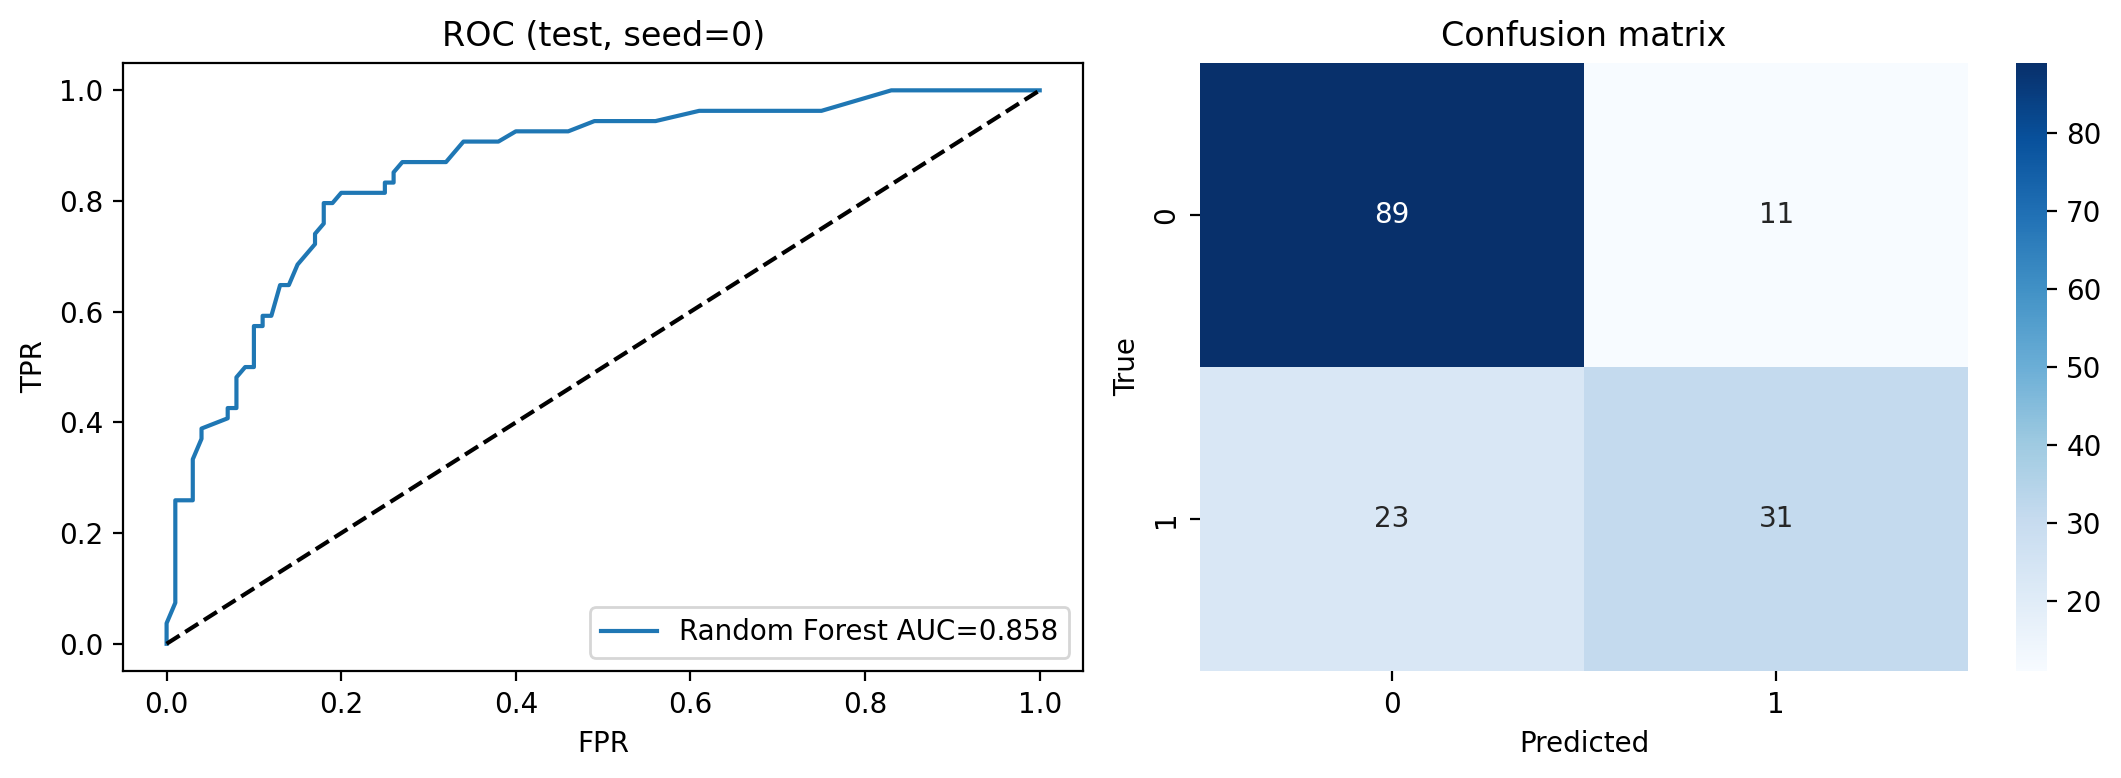
\includegraphics[width=\textwidth]{image/roc_confusion_test_seed0.png}
  \caption{Đường ROC (AUC $=0{,}858$) và ma trận nhầm lẫn trên tập kiểm thử: mô hình rừng ngẫu nhiên, \texttt{split\_seed=0} (TN=89, FP=11, FN=23, TP=31; $n_{\mathrm{test}}=154$).}
  \label{fig:roc-confusion}
\end{figure}

\subsection{Phân tích hiệu chuẩn xác suất \textnormal{(calibration analysis)}}
\label{subsec:calibration}

Ngoài hiệu năng phân loại, \textbf{chất lượng hiệu chuẩn} của xác suất dự đoán lớp dương được đánh giá bằng Brier score và đường hiệu chuẩn (Mục~\ref{subsec:metrics}). Bảng~\ref{tab:results-brier} báo cáo trung bình và độ lệch chuẩn của Brier trên \textbf{năm} lần chia train/test độc lập (cùng pipeline và script \texttt{resources/compute\_calibration.py}; artifact \texttt{brier\_mean\_std.csv}).

Brier càng nhỏ phản ánh xác suất dự đoán càng sát với nhãn thực theo nghĩa bình phương trung bình. Trong thực nghiệm này, \textbf{rừng ngẫu nhiên} có Brier trung bình thấp nhất, sát theo sau là \textbf{hồi quy logistic}; \textbf{SVM (RBF)} và \textbf{KNN} xếp tiếp theo, với SVM biến thiên hơn qua các seed (độ lệch chuẩn lớn hơn). Trên split đại diện (\texttt{split\_seed=0}), LR và RF gần như đồng hạng về Brier, phù hợp với đường hiệu chuẩn gần đường chéo trong Hình~\ref{fig:calibration}.
Kết hợp với ROC--AUC và PR--AUC cho thấy thứ hạng mô hình \textbf{không hoàn toàn nhất quán giữa các metric}: mô hình cạnh tranh tốt ở phân hạng chưa chắc đồng thời tối ưu ở hiệu chuẩn xác suất. Đây là lý do việc chọn metric cần bám mục tiêu tác vụ thay vì dùng một chỉ số duy nhất.

Hình~\ref{fig:calibration} vẽ đường hiệu chuẩn (10 bin, chiến lược \texttt{uniform}) cho bốn mô hình trên tập kiểm thử của split \texttt{split\_seed=0}. Đường nét đứt là hiệu chuẩn hoàn hảo ($y=x$). Hồi quy logistic và rừng ngẫu nhiên bám khá sát đường chéo ở nhiều bin; KNN dao động mạnh hơn do bản chất cục bộ và nhạy mẫu. Kết quả nhấn mạnh rằng \textbf{phân hạng mạnh} (ví dụ F1, ROC--AUC) và \textbf{xác suất hiệu chuẩn tốt} có thể đồng thời xuất hiện trên cùng một tập, song vẫn nên báo cáo riêng hai khía cạnh trong ứng dụng y tế.

\begin{table}[htbp]
  \centering
  \caption{Brier score (trung bình $\pm$ độ lệch chuẩn) qua năm lần chia train/test; nguồn \texttt{resources/outputs/latest/brier\_mean\_std.csv}.}
  \label{tab:results-brier}
  \begin{tabular}{lc}
    \toprule
    Mô hình & Brier (mean $\pm$ std) \\
    \midrule
    Random Forest         & $0{,}163 \pm 0{,}012$ \\
    Logistic Regression   & $0{,}165 \pm 0{,}013$ \\
    SVM (RBF)             & $0{,}171 \pm 0{,}023$ \\
    KNN                   & $0{,}183 \pm 0{,}014$ \\
    \bottomrule
  \end{tabular}
\end{table}

\begin{figure}[htbp]
  \centering
  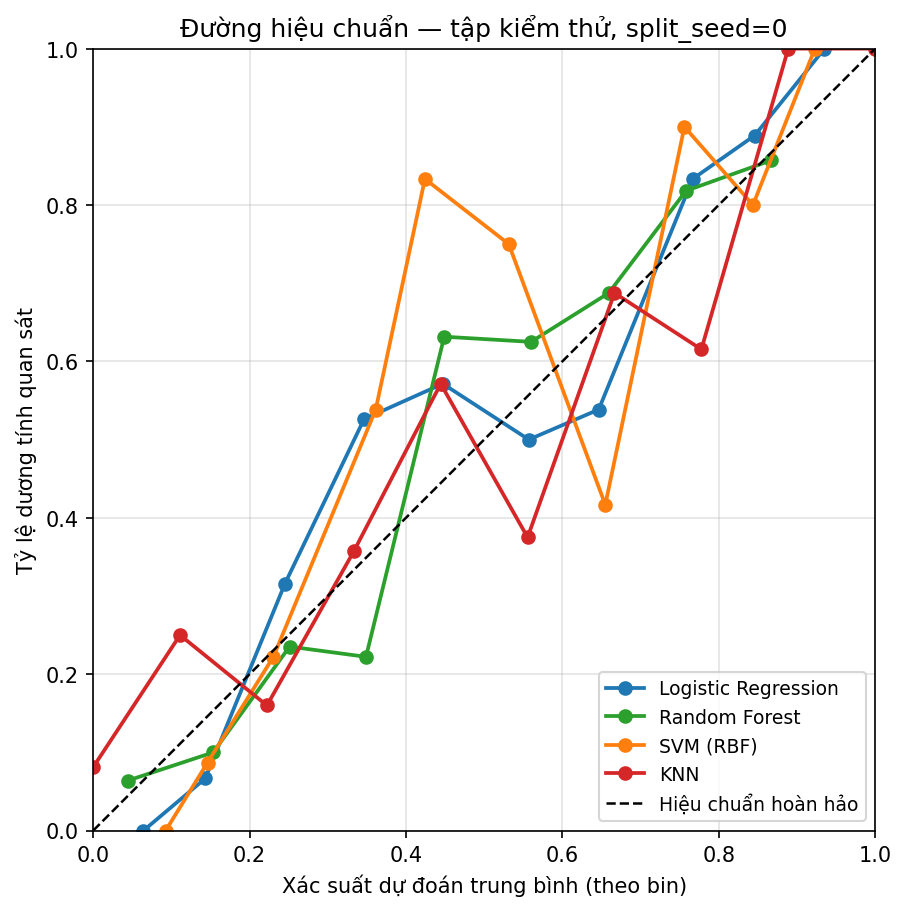
\includegraphics[width=0.72\textwidth]{image/calibration_curves_test_seed0.png}
  \caption{Đường hiệu chuẩn (reliability diagram) cho bốn mô hình trên tập kiểm thử, split đại diện \texttt{split\_seed=0}; đường nét đứt: hiệu chuẩn hoàn hảo.}
  \label{fig:calibration}
\end{figure}

\subsection{Đường Precision--Recall và PR--AUC \textnormal{(PR analysis)}}
\label{subsec:prauc}

Trong bối cảnh lớp dương tính chiếm tỷ lệ nhỏ hơn (Mục~\ref{subsec:dataset}), đường \textbf{Precision--Recall} và \textbf{PR--AUC} bổ sung cho ROC--AUC: PR nhấn mạnh đánh đổi giữa độ chính xác dương tính và độ nhạy trên lớp cần ưu tiên (Mục~\ref{subsec:metrics}). Bảng~\ref{tab:results-prauc} báo cáo PR--AUC trung bình $\pm$ độ lệch chuẩn qua năm lần chia (artifact \texttt{pr\_auc\_mean\_std.csv}).

\textbf{Rừng ngẫu nhiên} có PR--AUC trung bình cao nhất, tiếp theo là \textbf{hồi quy logistic}; \textbf{SVM (RBF)} và \textbf{KNN} xếp sau, với SVM độ lệch chuẩn lớn hơn, phù hợp với biến động đã thấy ở ROC--AUC. Hình~\ref{fig:pr-curves} vẽ đường Precision--Recall trên tập kiểm thử của \texttt{split\_seed=0}; đường ngang nét chấm là tỷ lệ dương tính trong tập kiểm thử (đường cơ sở của một bộ phân loại ngẫu nhiên theo tỷ lệ lớp). RF và LR tạo đường cong nằm gần phía trên so với KNN trên split này, phù hợp với PR--AUC trung bình.
Từ góc nhìn ``kể chuyện kết quả'', điểm quan trọng không chỉ là RF đứng đầu PR--AUC, mà là việc xếp hạng giữa các mô hình thay đổi theo chỉ số (AUC, PR--AUC, Brier), qua đó củng cố luận điểm rằng giao thức và metric có thể ảnh hưởng trực tiếp đến kết luận ``mô hình tốt nhất''.

\begin{table}[htbp]
  \centering
  \caption{PR--AUC (trung bình $\pm$ độ lệch chuẩn) qua năm lần chia train/test; nguồn \texttt{resources/outputs/latest/pr\_auc\_mean\_std.csv}.}
  \label{tab:results-prauc}
  \begin{tabular}{lc}
    \toprule
    Mô hình & PR--AUC (mean $\pm$ std) \\
    \midrule
    Random Forest         & $0{,}701 \pm 0{,}046$ \\
    Logistic Regression   & $0{,}692 \pm 0{,}050$ \\
    SVM (RBF)             & $0{,}672 \pm 0{,}097$ \\
    KNN                   & $0{,}615 \pm 0{,}057$ \\
    \bottomrule
  \end{tabular}
\end{table}

\begin{figure}[htbp]
  \centering
  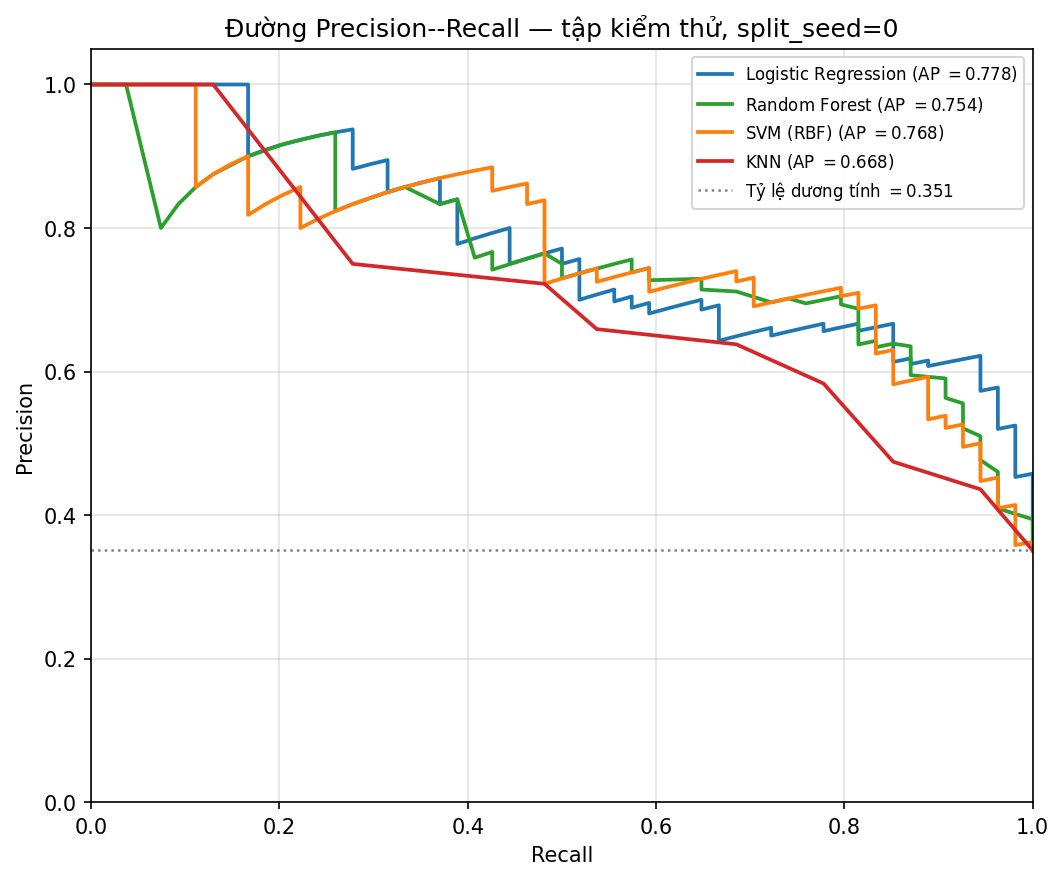
\includegraphics[width=0.72\textwidth]{image/pr_curves_test_seed0.png}
  \caption{Đường Precision--Recall cho bốn mô hình trên tập kiểm thử, \texttt{split\_seed=0} (chú thích: AP = PR--AUC trên tập đó). Đường nét chấm: tỷ lệ dương tính trong tập kiểm thử.}
  \label{fig:pr-curves}
\end{figure}

\subsection{Khoảng tin cậy bootstrap cho ROC--AUC và độ lớn hiệu ứng \textnormal{(uncertainty \& effect size)}}
\label{subsec:uncertainty-effect}

\textbf{Bất định ROC--AUC.} Bảng~\ref{tab:results-auc-bootstrap} trình bày ROC--AUC trên tập kiểm thử của \textbf{cùng} split đại diện (\texttt{split\_seed=0}) và khoảng tin cậy 95\% theo bootstrap ($B=1000$; Mục~\ref{subsec:metrics}). Khoảng của các mô hình dẫn đầu (LR, RF, SVM) \textbf{chồng lấn} đáng kể: chênh lệch điểm trung bình giữa các mô hình vì thế cần đọc kết hợp với độ biến thiên do chia tập (Bảng~\ref{tab:results-meanstd}), chứ không chỉ so trung bình đơn điệu.

\begin{table}[htbp]
  \centering
  \small
  \caption{ROC--AUC trên tập kiểm thử \texttt{split\_seed=0} và khoảng tin cậy 95\% (bootstrap có hoàn lại, $B=1000$). Nguồn: \texttt{resources/outputs/latest/roc\_auc\_bootstrap\_ci\_seed0.csv}.}
  \label{tab:results-auc-bootstrap}
  \begin{tabular}{lcc}
    \toprule
    Mô hình & ROC--AUC (split 0) & 95\% CI bootstrap \\
    \midrule
    Logistic Regression & $0{,}870$ & $[0{,}810\,;\,0{,}922]$ \\
    Random Forest       & $0{,}858$ & $[0{,}796\,;\,0{,}913]$ \\
    SVM (RBF)           & $0{,}855$ & $[0{,}788\,;\,0{,}917]$ \\
    KNN                 & $0{,}794$ & $[0{,}714\,;\,0{,}864]$ \\
    \bottomrule
  \end{tabular}
\end{table}

\textbf{Vì sao và khi nào (WHY + WHEN).} Việc các khoảng CI bootstrap của LR, RF và SVM chồng lấn đáng kể cho thấy chênh lệch ROC--AUC điểm ước lượng giữa các mô hình mạnh có thể không bền vững khi thay đổi mẫu kiểm thử. Trong các bối cảnh cần vận hành ổn định, kết quả này ủng hộ cách lựa chọn dựa trên \textbf{hồ sơ tổng thể} (hiệu năng + bất định + khả năng diễn giải) thay vì tối ưu một chỉ số đơn.

\textbf{Cliff's delta trên F1.} Bảng~\ref{tab:cliffs-delta} báo cáo Cliff's delta giữa các cặp mô hình (vector F1 theo năm seed; Mục~\ref{subsec:repro}). So sánh RF với LR và RF với SVM cho $|\hat{\delta}|$ \textbf{lớn} theo thang phổ biến (Mục~\ref{subsec:repro}), trong khi RF so với KNN chỉ đạt \textbf{nhỏ} ($\hat{\delta}=0{,}20$), phù hợp với kiểm định Wilcoxon không có ý nghĩa thống kê giữa RF và KNN (Mục~\ref{subsec:tablesfigures}). So sánh LR với KNN cho $\hat{\delta}=-0{,}24$ (nhỏ): theo định nghĩa, F1 của KNN có xu hướng lớn hơn F1 của LR trong một phần cấu hình cặp điểm trên năm split, phù hợp F1 trung bình gần nhau.

\textbf{Ý nghĩa thực tiễn của hiệu ứng.} Ở góc độ triển khai, các cặp có hiệu ứng \textbf{nhỏ} thường khó tạo khác biệt đáng kể trong vận hành hằng ngày và nên ưu tiên mô hình ổn định/dễ kiểm toán hơn; ngược lại, hiệu ứng \textbf{vừa/lớn} có thể là cơ sở hợp lý để cân nhắc đổi mô hình, nhưng vẫn cần đọc kèm yêu cầu giải thích, chi phí lỗi và độ ổn định theo split.

\begin{table}[htbp]
  \centering
  \small
  \caption{Cliff's delta (F1 theo năm \texttt{split\_seed}); \texttt{cliffs\_delta} $>0$ nghĩa là mô hình cột trái có xu hướng F1 cao hơn mô hình cột phải. Nguồn: \texttt{cliffs\_delta\_f1\_pairs.csv}.}
  \label{tab:cliffs-delta}
  \begin{tabular}{lcc}
    \toprule
    So sánh & $\hat{\delta}$ & Diễn giải (thang $|\cdot|$) \\
    \midrule
    RF vs LR   & $0{,}52$ & lớn \\
    RF vs KNN  & $0{,}20$ & nhỏ \\
    RF vs SVM  & $0{,}52$ & lớn \\
    LR vs SVM  & $0{,}48$ & lớn \\
    LR vs KNN  & $-0{,}24$ & nhỏ \\
    SVM vs KNN & $-0{,}36$ & vừa \\
    \bottomrule
  \end{tabular}
\end{table}

\subsection{Phân tích độ quan trọng đặc trưng \textnormal{(permutation importance)}}
\label{subsec:permimp}

Mục này bổ sung giải thích \textbf{agnostic} (Mục~\ref{subsec:interpret}): với mỗi lần chia train/test và mỗi mô hình đã huấn luyện, \texttt{permutation\_importance} đo \textbf{suy giảm F1} trên tập kiểm thử khi hoán vị từng đặc trưng ($n_{\mathrm{rep}}=30$); kết quả được \textbf{trung bình qua năm seed} và trình bày theo mô hình trong Hình~\ref{fig:perm-importance}.

Trên tổng thể các mô hình và split, \textbf{Glucose} và \textbf{BMI} có độ quan trọng hoán vị trung bình cao nhất; tiếp theo là \textbf{Age} và, ở mức thấp hơn, \textbf{Insulin}. Một số biến (ví dụ huyết áp, độ dày da) cho trung bình gần $0$ hoặc \textbf{âm nhỏ}; hiện tượng này có thể xuất hiện khi cỡ mẫu kiểm thử hạn chế và khi xáo trộn giảm nhiễu ngẫu nhiên hơn là phá cấu trúc hữu ích, nên cần đọc thận trọng cùng hệ số LR và độ quan trọng RF (artifact gốc). Thứ hạng đỉnh (Glucose, BMI) \textbf{ổn định} qua các cách chia tập, gợi ý không chỉ là artifact của một phân hoạch may mắn.

So sánh nhanh: thứ hạng impurity của RF và hệ số LR trên split đại diện (RQ2) \textbf{nhất quán} với permutation về các biến chủ đạo; chỗ lệch nhỏ giữa các phép đo là điều dự kiến khi impurity thiên lệch với tương quan biến.

\begin{table}[htbp]
  \centering
  \small
  \caption{Trung bình độ quan trọng hoán vị (trước hết trung bình trên bốn mô hình tại mỗi seed, rồi trung bình trên năm seed; đơn vị: suy giảm F1). Nguồn: \texttt{permutation\_importance\_consensus.csv}.}
  \label{tab:perm-consensus}
  \begin{tabular}{lcc}
    \toprule
    Đặc trưng & Trung bình & Độ lệch chuẩn (qua seed) \\
    \midrule
    Glucose & $0{,}168$ & $0{,}018$ \\
    BMI & $0{,}038$ & $0{,}020$ \\
    Age & $0{,}012$ & $0{,}015$ \\
    Insulin & $0{,}005$ & $0{,}006$ \\
    \bottomrule
  \end{tabular}
\end{table}

\begin{figure}[htbp]
  \centering
  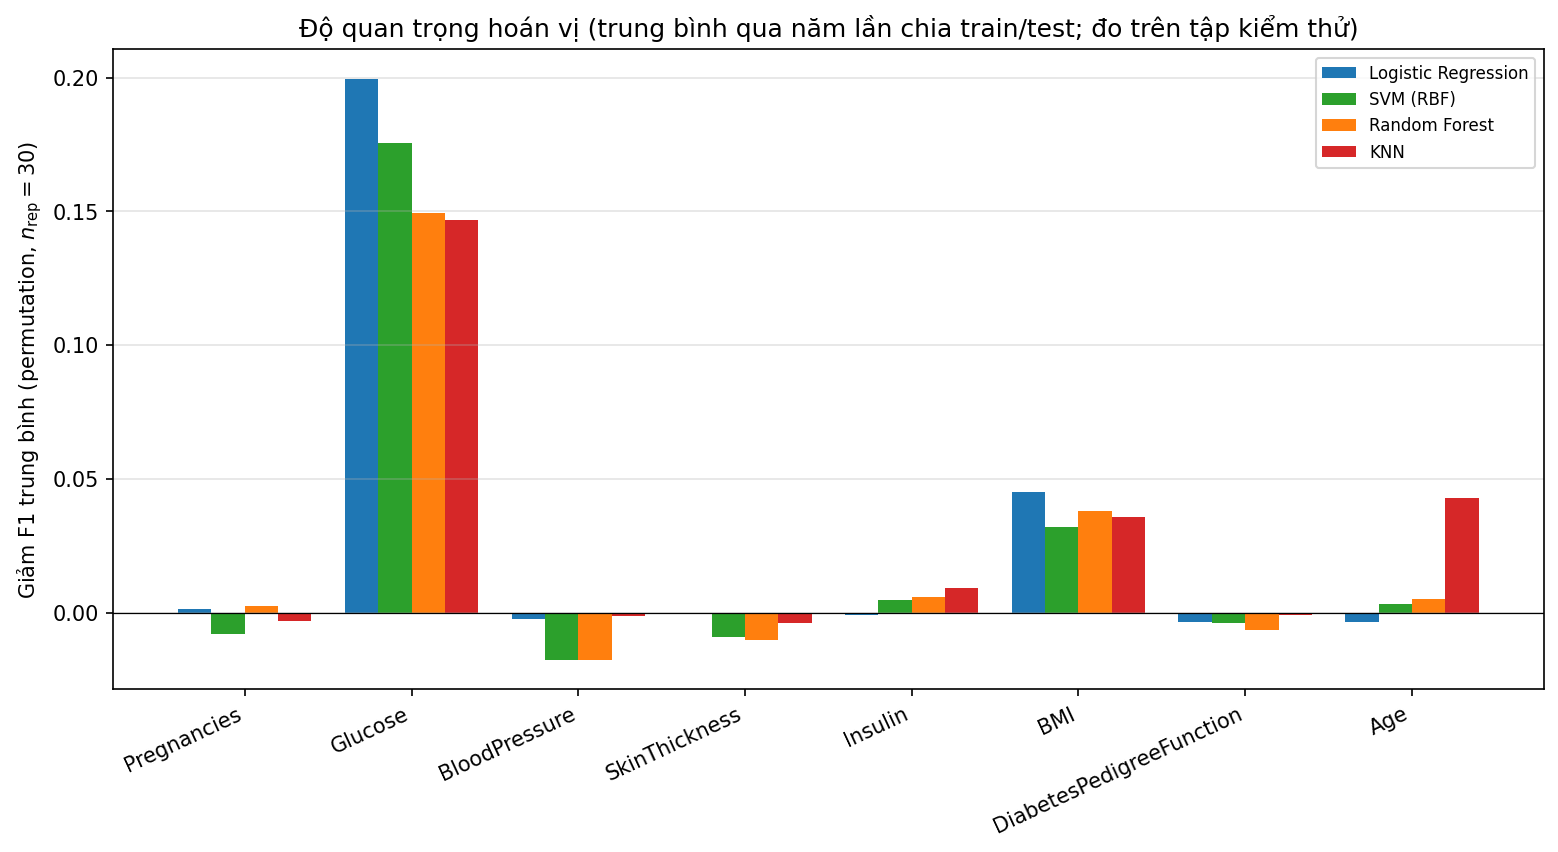
\includegraphics[width=\textwidth]{image/permutation_importance_mean5splits.png}
  \caption{Suy giảm F1 trung bình do hoán vị từng đặc trưng (permutation importance, $n_{\mathrm{rep}}=30$), đo trên \textbf{tập kiểm thử}, trung bình qua năm lần chia train/test; bốn mô hình học.}
  \label{fig:perm-importance}
\end{figure}

\subsection{Nghiên cứu loại bỏ \textnormal{(ablation study)}}
\label{subsec:ablation}

Mục này bổ sung cho kết quả chính (Mục~\ref{subsec:tablesfigures}) bằng cách \textbf{kiểm tra có điều kiện} đóng góp của một thành phần pipeline, ở đây là \textbf{chuẩn hóa đặc trưng}, và nhắc lại vai trò \textbf{lý thuyết và phương pháp} của các bước còn lại đã cố định trong toàn bộ thực nghiệm (Mục~\ref{sec:methods}). Mục tiêu không phải lặp lại toàn bộ lưới siêu tham số mà là tránh hiểu nhầm rằng hiệu năng chỉ đến từ một ``mẹo'' đơn lẻ ngoài bối cảnh giao thức đã thống nhất.

\textbf{Thí nghiệm có số liệu xuất artifact.} Trên \textbf{một} split giữ nguyên (\texttt{split\_seed=0}), so sánh hai pipeline hồi quy logistic với \textbf{cùng} \texttt{C=1{,}0} cố định: (i) điền thiếu + \texttt{StandardScaler}; (ii) chỉ điền thiếu, \textbf{không} chuẩn hóa. Kết quả trên tập kiểm thử (file \texttt{resources/outputs/latest/ablation\_lr\_scaler.csv}) cho thấy F1 \textbf{trùng khớp} tới nhiều chữ số thập phân ($\approx 0{,}624$). Điều này cho thấy, \emph{với mức điều chuẩn cố định này và trên split đã chọn}, bước Z-score không đổi điểm F1 được báo cáo; tuy nhiên, \textbf{không} thể suy ra rằng chuẩn hóa luôn thừa cho hồi quy logistic. Khi \texttt{C} được chọn bằng \texttt{GridSearchCV} trên lưới (Phụ lục~\ref{app:hyper}), thang đo đặc trưng và mức điều chuẩn có tương tác; ablation đầy đủ theo từng giá trị \texttt{C} nằm ngoài phạm vi đoạn so sánh tối giản này và đã được xử lý trong luồng huấn luyện chính.

\textbf{Tiền xử lý và các mô hình nhạy thang đo.} Đối với KNN và SVM (RBF), co giãn đặc trưng là \textbf{yếu tố cấu thiết} về mặt lý thuyết vì quyết định phụ thuộc khoảng cách hoặc margin trong không gian gốc (Mục~\ref{subsec:preprocess}). Luận văn \textbf{không} báo cáo thêm bảng ``bỏ scaler'' riêng cho từng mô hình này, vì kết quả chính luôn dùng \textbf{cùng} pipeline imputer+scaler; việc bỏ chuẩn hóa được kỳ vọng làm suy giảm mạnh hiệu năng và không phản ánh giao thức đề xuất. \emph{Cách đọc ablation:} ablation có số liệu chỉ đối chứng LR với/không Z-score tại một \texttt{C} cố định (Mục trên); từ đó \textbf{không} kết luận ``ai giảm nhiều nhất khi bỏ scaler'' bằng bảng mới. Thay vào đó, theo lý thuyết học máy, \textbf{KNN và SVM} là hai họ \textbf{nhạy cực đại} với độ lớn đặc trưng nên được kỳ vọng là \textbf{chịu sụt giảm lớn nhất} nếu bỏ chuẩn hóa; RF và LR (đặc biệt khi \texttt{C} đã được chọn lại trên lưới) có thể kém nhạy hơn ở mức khác nhau. Đây là \textbf{giải thích có căn cứ lý thuyết} bổ sung cho con số LR--scaler đã có, chứ không thay thế một bảng ablation đầy đủ cho mọi mô hình.

\textbf{Tinh chỉnh siêu tham số.} Toàn bộ mô hình học trong Bảng~\ref{tab:results-point}--\ref{tab:results-meanstd} đều qua \texttt{GridSearchCV} như Mục~\ref{subsec:training}. Không tách riêng một bảng ``không tinh chỉnh'' trong luận văn vì đường cơ sở phương pháp đã coi tinh chỉnh là \textbf{bộ phận không tách rời} của so sánh công bằng; mặc định thư viện với siêu tham số tùy ý thường kém ổn định và khó đối chiếu với lưới đã công bố. \emph{Ý nghĩa ``câu chuyện'':} nếu \textbf{bỏ bước xác thực chéo nội bộ} và cố định siêu tham số kém phù hợp, phương sai ước lượng hiệu năng và \textbf{dao động thứ hạng} giữa các lần chia tập thường \textbf{tăng}---đúng với những gì độc giả thấy khi so Bảng~\ref{tab:results-point} (một split) với Bảng~\ref{tab:results-meanstd} (năm split) trong cùng giao thức đã tinh chỉnh.

\textbf{Giao thức đánh giá (một split so với nhiều seed).} Sự \emph{khác biệt} giữa Bảng~\ref{tab:results-point} (một lần chia) và Bảng~\ref{tab:results-meanstd} (năm lần) minh họa trực quan mức \textbf{dao động} khi chỉ đổi \texttt{random\_state}; đây cũng là lý do báo cáo trung bình $\pm$ độ lệch chuẩn và CI (Mục~\ref{subsec:protocol}). Đây là đối chứng phương pháp cho rủi ro kết luận từ \textbf{một} split may mắn, không cần thêm thí nghiệm tách file: \emph{một} đường đánh giá duy nhất dễ \textbf{phóng đại hoặc đảo thứ hạng} so với trung bình trên nhiều phân hoạch.

\textbf{Baseline.} \texttt{DummyClassifier} (đa số) không bị ``loại khỏi'' bài toán mà luôn có mặt trong cùng bảng kết quả, cung cấp \textbf{mốc tối thiểu} và ngữ cảnh cho Precision/Recall/F1 (Mục~\ref{subsec:models}). Bỏ baseline khỏi báo cáo sẽ làm mất đối chiếu với chiến lược tầm thường.

\noindent\textit{Tóm lại,} ablation có mã và CSV minh họa nhấn mạnh giới hạn của một so sánh cố định \texttt{C} khi bàn về vai trò scaler đối với LR; đồng thời kể một \textbf{chuỗi nhân quả phương pháp} (scaler $\rightarrow$ KNN/SVM nhạy nhất; inner CV $\rightarrow$ giảm phương sai siêu tham số; nhiều seed $\rightarrow$ bớt ảo giác thứ hạng từ một lần chia). Các thành phần còn lại của pipeline, gồm chuẩn hóa đối với KNN/SVM, \texttt{GridSearchCV}, lặp nhiều seed, baseline đa số, được củng cố bằng lý thuyết và bằng cấu trúc bảng kết quả đã trình bày, phù hợp phạm vi một luận văn ưu tiên tái lập và minh bạch hơn là quét mọi tổ hợp ablation độc lập.

\textbf{Kết đoạn Results (trade-off).} Tổng hợp các tiểu mục từ Bảng~\ref{tab:results-point} đến Mục~\ref{subsec:ablation} cho thấy một đánh đổi nhất quán giữa \textbf{hiệu năng cực đại} và \textbf{độ ổn định}. RF thường đạt lợi thế ở các chỉ số phân loại chính, nhưng LR cho hồ sơ ổn định và diễn giải trực tiếp hơn. Do đó, không có mô hình tối ưu tuyệt đối cho mọi mục tiêu: lựa chọn cuối cùng cần gắn với ưu tiên ứng dụng (tối đa hóa hiệu năng hay ưu tiên ổn định và khả năng giải thích). Phần Discussion tiếp theo mở rộng các hàm ý này dưới góc nhìn phương pháp và ứng dụng.

\section{Thảo luận}
\label{sec:discussion}

\noindent Phần này tập trung \textbf{diễn giải cơ chế} đằng sau các quan sát thực nghiệm thay vì lặp lại bảng số liệu. Trục phân tích chính gồm ba câu hỏi: \textbf{(i) vì sao} các mô hình cho hành vi khác nhau, \textbf{(ii) khi nào} mỗi mô hình phù hợp hơn theo điều kiện dữ liệu và mục tiêu tác vụ, và \textbf{(iii) đánh đổi nào} cần chấp nhận giữa hiệu năng, độ ổn định và khả năng diễn giải.

\subsection{Phân tích kết quả \textnormal{(discussion of results)}}
\label{subsec:disc-results}

Các luận điểm dưới đây liên kết trực tiếp số liệu ở Mục~\ref{sec:results} với giả định học thống kê của từng họ mô hình, nhằm chuyển từ ``xếp hạng chỉ số'' sang ``giải thích cơ chế'' trong cùng giao thức thực nghiệm. Mạch lập luận được trình bày theo chuỗi: \textbf{quan sát kết quả} $\rightarrow$ \textbf{giải thích cơ chế} $\rightarrow$ \textbf{hàm ý ứng dụng} $\rightarrow$ \textbf{giới hạn khái quát}.

\textbf{Hành vi mô hình và khác biệt hiệu năng.}
\textbf{Rừng ngẫu nhiên} đạt F1 trung bình cao nhất (Bảng~\ref{tab:results-meanstd}), phù hợp với khả năng của \textbf{tổ hợp cây} trong nắm bắt \textbf{tương tác phi tuyến} giữa các đặc trưng: trên tập Pima, quan hệ giữa các biến lâm sàng (đường huyết, BMI, tuổi và tiền sử gia đình) khó được mô tả đầy đủ bằng một ranh giới tuyến tính đơn; phân tách phân cấp theo cây có thể khai thác các tương tác đó, cải thiện recall và cân bằng Precision--F1 trên một số phân hoạch. \emph{Điểm then chốt:} cả hệ số LR và permutation importance đều xếp \textbf{Glucose} và \textbf{BMI} lên hàng đầu; RF có thể mô hình hóa \textbf{kết hợp điều kiện} (ví dụ vùng ``glucose cao \emph{và} BMI cao'') mà một mặt phẳng log-odds tuyến tính không diễn đạt hết, góp phần giải thích vì sao RF thường nhích hơn về F1 trong khi vẫn chịu dao động giữa các split.

Ngược lại, \textbf{hồi quy logistic} giả định quan hệ \textbf{tuyến tính trong không gian log-odds}; giả định này có thể giới hạn khả năng bắt mẫu phức tạp, nhưng đồng thời tạo \textbf{inductive bias} mạnh hơn, giúp kiểm soát phương sai, đặc biệt khi cỡ mẫu hạn chế. Điều này củng cố kết quả quan sát: LR có Accuracy và ROC--AUC trung bình cao nhất (Bảng~\ref{tab:results-meanstd}), phù hợp với khả năng \textbf{xếp hạng toàn cục} (ranking) ổn định trên toàn bộ phổ xác suất dự đoán khi ranh giới tuyến tính vẫn tách lớp khá tốt trong không gian đã chuẩn hóa; độ lệch chuẩn F1 của LR còn \textbf{nhỏ hơn} RF ($0{,}017$ so với $0{,}025$), gợi ý \textbf{ổn định} hơn qua các cách chia tập ở tiêu chí này. Nói gọn, có một \textbf{đánh đổi}: RF nhích về F1 nhờ cấu trúc phi tuyến, LR nhích về AUC/ổn định nhờ mô hình đơn giản hơn dưới mẫu nhỏ---đúng với mẫu hình thường gặp trên dữ liệu y sinh dạng bảng cỡ hạn chế.

\textbf{Đánh đổi thiên kiến--phương sai.}
Sự khác biệt có thể đọc qua thấu kính \textbf{bias--variance}: LR là mô hình đơn giản hơn (thiên kiến cao hơn, phương sai thường thấp hơn), thường \textbf{vững hơn} khi dữ liệu hạn chế; RF linh hoạt hơn, có thể phù hợp đặc trưng phi tuyến nhưng phụ thuộc nhiều vào các phân tách dữ liệu mang tính cục bộ và có thể dao động mạnh hơn giữa các lần chia. Trên năm split, RF có F1 trung bình cao hơn nhưng không ``êm'' hơn LR về độ lệch chuẩn F1; điều này minh họa đánh đổi giữa đỉnh hiệu năng trung bình và \textbf{tính lặp lại} giữa các phân hoạch.

\textbf{Khi nào ưu tiên mô hình nào.}
Lựa chọn nên gắn với \textbf{ngữ cảnh ứng dụng} chứ không một chỉ số đơn lẻ: RF thích hợp khi ưu tiên tối đa hóa F1/recall trên lớp dương và chấp nhận mô hình có nhiều tham số hơn; LR thích hợp khi cần \textbf{minh bạch} hệ số theo biến, ổn định qua split, và lộ trình kiểm chứng đơn giản. Điều này đặc biệt quan trọng trong bối cảnh lâm sàng khi cần giải thích có kiểm soát. Các hàm ý triển khai và lựa chọn mô hình lưu được làm rõ thêm ở Mục~\ref{subsec:disc-implications}.

Kết quả Mục~\ref{sec:results} cho thấy \textbf{chênh lệch hiệu năng giữa các mô hình là tương đối nhỏ} dù RF đạt F1 trung bình cao nhất qua năm lần chia tập (Bảng~\ref{tab:results-meanstd}). Kiểm định \textbf{Wilcoxon signed-rank} trên F1 theo từng split giữa RF và KNN (hai mô hình có F1 trung bình cao) cho $p\approx 0{,}44$ (Mục~\ref{subsec:tablesfigures}), nên \textbf{không} có cơ sở thống kê mạnh để khẳng định một thuật toán ``vượt trội'' ở mức ý nghĩa thông thường với $n=5$ split. \textbf{Lưu ý phương pháp:} với chỉ \textbf{năm} cặp điểm ghép, \textbf{lực thống kê} (statistical power) của Wilcoxon thấp; \emph{thiếu ý nghĩa thống kê} vì thế \textbf{không} đồng nghĩa chứng minh hai phân bố F1 bằng nhau, mà chỉ cho thấy bằng chứng trong thiết lập này \textbf{chưa đủ mạnh} để bác bỏ giả thuyết không. Điều này củng cố cách đọc: \emph{ưu thế quan sát được} có thể chịu ảnh hưởng đáng kể từ \textbf{biến thiên do cách chia tập} và từ phương sai ước lượng khi cỡ mẫu hạn chế.

Về các mô hình còn lại, \textbf{KNN} dựa trên \textbf{láng giềng cục bộ} trong không gian đặc trưng nên vừa \textbf{nhạy với chuẩn hóa thang đo} vừa nhạy với \textbf{mật độ cục bộ} và nhiễu nhãn ở vùng biên; trên mẫu vừa phải, một vài điểm kiểm thử thay đổi theo split có thể làm đổi láng giềng đa số, dẫn tới \textbf{dao động} giữa các seed (Bảng~\ref{tab:results-meanstd}) dù pipeline đã dùng imputer+scaler thống nhất. \textbf{SVM (RBF)} tối ưu \textbf{biên tách lớp} trong không gian nhân; hiệu năng phụ thuộc cặp $(C,\gamma)$ đã chọn và vẫn chịu ảnh hưởng từ \textbf{cấu trúc cục bộ} của dữ liệu sau ánh xạ, nên cũng có thể biến động qua các phân hoạch train/test khác nhau. Trong pipeline thống nhất, hai mô hình này đạt mức cạnh tranh trên một số split (Bảng~\ref{tab:results-point}), song thứ hạng trung bình phụ thuộc lưới và có xu hướng \textbf{biến động} hơn so với LR (Bảng~\ref{tab:results-meanstd}), phù hợp kỳ vọng phương sai cao hơn khi cỡ mẫu vừa phải.

\textbf{Trả lời RQ1.} Theo F1 trung bình, RF dẫn ($0{,}614 \pm 0{,}025$), tiếp theo KNN và LR; SVM (RBF) thấp hơn trong lưới đã dùng. Accuracy và ROC--AUC trung bình cao nhất thuộc LR ($0{,}748 \pm 0{,}018$; $0{,}824 \pm 0{,}031$). Trên split đại diện (Bảng~\ref{tab:results-point}), SVM và RF có F1 gần bằng ($\approx 0{,}646$) và cao hơn LR; điều này minh họa \textbf{đánh đổi} giữa tiêu chí (F1 so với AUC) và \textbf{độ nhạy với seed}.

\textbf{Trả lời RQ2.} Trên mô hình đã huấn luyện (\texttt{split\_seed=0}), \textbf{Glucose} và \textbf{BMI} có hệ số LR (không gian đã scale) và độ quan trọng RF lớn nhất; tiếp theo là tuổi và chỉ số phả hệ đái tháo đường (\texttt{lr\_coefficients\_scaled\_space.csv}, \texttt{rf\_feature\_importance.csv}). \textbf{Permutation importance} trung bình qua năm split (Mục~\ref{subsec:permimp}) củng cố Glucose và BMI là hai biến có tác động mạnh nhất theo cách đo agnostic. Thứ tự này phù hợp kiến thức lâm sàng về đường huyết và béo phì trong nguy cơ đái tháo đường type 2, nhưng chỉ mang tính hỗ trợ giải thích, không suy ra nhân quả.\cite{kirbas2025shap,chang2022pima}

\textbf{Phân hạng so với hiệu chuẩn xác suất.}
Một điểm cần tách bạch là \textbf{khả năng phân tách} (discrimination) và \textbf{độ tin cậy của xác suất} (calibration). Trong lý thuyết học máy, mô hình có ranh giới quyết định linh hoạt hơn có thể đạt F1 cao nhưng xác suất kém hiệu chuẩn; ngược lại, mô hình tuyến tính thường được coi là ứng viên tự nhiên cho xác suất dễ diễn giải hơn, nhưng điều đó \textbf{không} đảm bảo Brier tốt hơn trên mọi tập. Trên tập và giao thức này, rừng ngẫu nhiên vừa dẫn đầu F1 trung bình (Bảng~\ref{tab:results-meanstd}) vừa có Brier trung bình thấp nhất (Bảng~\ref{tab:results-brier}), trong khi hồi quy logistic đứng thứ hai về cả hai khía cạnh ở mức \textbf{sát nhau}. Điều này minh họa rằng hai tiêu chí không luôn mâu thuẫn, nhưng cũng \textbf{không} suy ra lẫn nhau; vì vậy việc báo cáo Brier và đường hiệu chuẩn (Mục~\ref{subsec:calibration}) vẫn cần thiết khi xác suất được dùng cho phân tầng nguy cơ hoặc ngưỡng quyết định. Nếu ưu tiên diễn giải hệ số tuyến tính và minh bạch tham số, LR vẫn là lựa chọn hợp lý dù F1 trung bình thấp hơn RF một chút.

\textbf{Độ vững của chênh lệch hiệu năng.} Bổ sung PR--AUC (Mục~\ref{subsec:prauc}) làm rõ hiệu năng trên lớp dương tính trong bối cảnh mất cân bằng nhẹ; RF và LR vẫn dẫn đầu theo PR--AUC trung bình, phù hợp với các chỉ số khác. \textbf{Khoảng tin cậy bootstrap} cho ROC--AUC trên một tập kiểm thử cố định (Bảng~\ref{tab:results-auc-bootstrap}) chồng lấn giữa các mô hình mạnh, nhắc rằng chênh lệch điểm trung bình \textbf{không} tự khẳng định ưu thế tuyệt đối khi khoảng ước lượng bất định rộng. \textbf{Cliff's delta} (Bảng~\ref{tab:cliffs-delta}) cho thấy một số cặp có hiệu ứng ``lớn'' theo thang $|\hat{\delta}|$, trong khi RF so với KNN chỉ \textbf{nhỏ}, phù hợp với Wilcoxon không phát hiện khác biệt có ý nghĩa trên F1. Tổng thể, cần đọc song song \emph{ý nghĩa thống kê}, \emph{khoảng tin cậy} và \emph{độ lớn hiệu ứng}, tránh phóng đại cải tiến biên độ hẹp trên cỡ mẫu vừa phải.

\textbf{Claim--evidence--implication.} Từ các bằng chứng trên (dao động theo split, chồng lấn CI, và hiệu ứng nhỏ ở một số cặp), hàm ý phương pháp là: lựa chọn mô hình trong dữ liệu y sinh nhỏ nên ưu tiên \textbf{độ vững của quy trình đánh giá} trước khi ưu tiên chênh lệch điểm số biên.

\textbf{P-value và ý nghĩa thực tiễn.} Một điểm phương pháp quan trọng là khác biệt ``có ý nghĩa thống kê'' chưa chắc kéo theo khác biệt ``đáng kể trong vận hành''. Vì vậy, quyết định chọn mô hình ở đây được đặt trên tổ hợp bằng chứng gồm p-value, hiệu ứng thực tế và mức ổn định qua seed, thay vì suy luận từ một tiêu chí đơn lẻ.

\textbf{Độ vững của thứ hạng đặc trưng.} Việc bổ sung \textbf{permutation importance} (Mục~\ref{subsec:permimp}) củng cố phân tích giải thích: đây là đo \textbf{agnostic} ít phụ thuộc cấu trúc mô hình hơn impurity của RF, nên giảm rủi ro ``thổi phồng'' một biến chỉ vì cây cắt nhiều trên biến đó. Sự nhất quán giữa hệ số LR, độ quan trọng RF và permutation về vai trò của Glucose và BMI tăng độ tin cậy định tính cho RQ2; các lệch nhỏ giữa impurity và hoán vị vẫn có thể xuất hiện khi biến tương quan. Đây cũng là lý do khuyến nghị \textbf{đa phương pháp} trong giải thích y sinh.

\textbf{Đặc điểm lỗi và ranh giới quyết định.}
Phân tích định tính gợi ý rằng \textbf{false negative} thường tập trung ở các \textbf{trường hợp biên}, tức một số đặc trưng gần ranh giới quyết định, nơi mô hình linh hoạt như RF có thể thích nghi hơn so với ranh giới tuyến tính của LR, góp phần vào recall tốt hơn trên một số phân hoạch. Tuy nhiên, độ linh hoạt cũng có thể làm tăng \textbf{false positive} nhất định, phản ánh đánh đổi độ nhạy--độ đặc hiệu. LR với ranh giới mượt hơn trong không gian log-odds có thể ít cực đoan hơn ở một số vùng nhưng bỏ sót mẫu phi tuyến tinh vi. Số liệu ma trận nhầm lẫn trên một split đại diện được trình bày ở Mục~\ref{subsec:disc-error-related} (Hình~\ref{fig:roc-confusion}).

\textbf{Từ ma trận nhầm lẫn đến hệ quả trong sàng lọc \textnormal{(healthcare-aware reading)}.}
Trong nhiều kịch bản sàng lọc, \textbf{false negative} (bỏ sót ca thật dương tính) đặc biệt nặng vì có thể \textbf{trì hoãn theo dõi và điều trị}, làm tăng nguy cơ biến chứng; \textbf{false positive} chủ yếu gây \textbf{xét nghiệm bổ sung, tái khám và gánh nặng tâm lý/chi phí}, tùy bối cảnh tổ chức. Vì vậy, đọc FP/FN không chỉ là đọc số trên bảng mà là gắn với \textbf{hàm chi phí ưu tiên} của từng chương trình sàng lọc---và với lưu ý luận văn chỉ minh họa phương pháp, không thay thế quy trình lâm sàng.

\textbf{Tóm lại kết quả thảo luận.}
Không có mô hình đơn lẻ nào dẫn đầu đồng thời mọi tiêu chí: RF thể hiện phân loại mạnh (F1, PR--AUC), trong khi LR mang lại độ ổn định và khả năng phân tách (AUC) cùng cấu trúc giải thích rõ ràng; cả hai đều cần đọc kèm hiệu chuẩn và bất định thống kê. Điều này củng cố cách đánh giá \textbf{đa chiều} thay vì một chỉ số duy nhất.

\textbf{Hàm ý khái quát hóa ở mức nghiên cứu.} Một quan sát quan trọng là khác biệt hiệu năng giữa các mô hình phụ thuộc không chỉ vào bản thân thuật toán mà còn phụ thuộc mạnh vào đặc tính dữ liệu và giao thức đánh giá. Vì vậy, kết luận về ``mô hình tốt nhất'' trong một nghiên cứu đơn lẻ cần được diễn giải thận trọng, do thứ hạng có thể thay đổi khi chuyển sang tập dữ liệu hoặc thiết lập đánh giá khác. Theo hướng đó, giá trị bền vững hơn là xây dựng quy trình đánh giá chuẩn hóa, tái lập được và chống rò rỉ, để so sánh công bằng các phương pháp trong từng bối cảnh cụ thể.

Ở mức rộng hơn, mẫu hình kết quả này nhiều khả năng cũng xuất hiện trên các bộ dữ liệu y sinh dạng bảng quy mô nhỏ khác, nơi tương tác đặc trưng tồn tại nhưng kích thước mẫu còn hạn chế: mô hình linh hoạt thường đạt đỉnh hiệu năng cao hơn, trong khi mô hình đơn giản hơn cho độ ổn định tốt hơn. Dù vậy, mức độ chuyển giao vẫn cần được xác nhận bằng external validation trước khi khái quát ra quần thể mới.

\subsection{Hàm ý thực tiễn \textnormal{(practical implications)}}
\label{subsec:disc-implications}

Tiếp nối phân tích hành vi mô hình (Mục~\ref{subsec:disc-results}), trong bối cảnh chỉ số \textbf{không} có mô hình thắng đồng thời trên mọi tiêu chí, việc \textbf{chọn mô hình} nên gắn với \textbf{ưu tiên tác vụ}: nếu nhấn mạnh F1 trên lớp dương và khả năng nắm cấu trúc phi tuyến, RF là lựa chọn hợp lý và khớp với mô hình được lưu theo F1 trung bình (\texttt{resources/diabetes\_prediction\_model.pkl}); nếu ưu tiên \textbf{minh bạch} và diễn giải hệ số theo biến, LR thường thuận tiện hơn, đồng thời đạt ROC--AUC trung bình cao. Sự chênh lệch nhỏ giữa các thuật toán dẫn đầu cũng gợi ý rằng \textbf{chi phí tính toán}, \textbf{thời gian huấn luyện}, \textbf{khả năng triển khai} (ví dụ suy luận nhanh, kiểm định phần mềm) có thể đóng vai trò quyết định thực tế ngang với chênh lệch chỉ số trong phạm vi thống kê mơ hồ.

\textbf{Gợi ý lựa chọn ở mức quyết định \textnormal{(decision-level insight)}.}
Trong kịch bản \textbf{sàng lọc sớm} mà ưu tiên giảm \textbf{bỏ sót ca dương tính} (tức coi trọng recall/độ nhạy), các mô hình có xu hướng đạt F1/recall cao hơn trên giao thức đã báo cáo---điển hình \textbf{rừng ngẫu nhiên} trong luận văn---thường là hướng ưu tiên \emph{để thử nghiệm tiếp} trong pipeline minh họa, kèm điều chỉnh ngưỡng theo chi phí lâm sàng. Ngược lại, khi ưu tiên \textbf{tính giải thích, kiểm toán quyết định và độ ổn định} qua nhiều lần chia tập, \textbf{hồi quy logistic} là lựa chọn thay thế \emph{đáng tin cậy hơn} nhờ hệ số đọc được và ROC--AUC trung bình dẫn đầu trong thiết lập này. Đây không phải khuyến cáo lâm sàng mà là \textbf{khung ra quyết định phương pháp}: gắn thuật toán với \emph{mục tiêu vận hành} (giảm FN so với kiểm soát FP, hoặc ngược lại) trước khi cố định triển khai.

Về \textbf{ứng dụng y tế}, mọi mô hình ở đây chỉ mang tính \textbf{hỗ trợ nghiên cứu hoặc giáo dục}, không thay thế chẩn đoán lâm sàng; triển khai thực tế cần quy trình xác thực độc lập, quản trị rủi ro và tuân thủ bảo vệ dữ liệu (xem Mục~\ref{subsec:disc-limitations}).

\textbf{Khuyến nghị thực tiễn.} Từ các kết quả hiện tại, có thể rút ra hai nguyên tắc triển khai: (i) trong các tác vụ sàng lọc ưu tiên giảm bỏ sót ca dương tính, có thể ưu tiên mô hình/thiết lập đạt recall cao hơn dù phải đánh đổi một phần precision; (ii) trong bối cảnh cần minh bạch và \textbf{kiểm toán quyết định}, các mô hình tuyến tính như LR thường phù hợp hơn nhờ khả năng diễn giải trực tiếp. Đồng thời, mọi quyết định nên dựa trên đánh giá qua \textbf{nhiều lần chia dữ liệu}, thay vì một split duy nhất, để giảm rủi ro kết luận do ngẫu nhiên.

Ở mức triển khai quy trình, nên tách riêng hai bước: \textbf{chọn mô hình} theo giao thức tái lập (nhiều split) và \textbf{chọn ngưỡng quyết định} theo hàm chi phí lâm sàng của từng đơn vị (chi phí FN so với FP). Với LR, các hệ số còn có thể chuyển thành thang điểm (hoặc nomogram) để hỗ trợ truyền thông nguy cơ một cách minh bạch trong thực hành.

\textbf{Decision guideline (tóm tắt).}
\begin{itemize}
  \item Nếu ưu tiên \textbf{diễn giải và kiểm toán}: ưu tiên LR.
  \item Nếu ưu tiên \textbf{hiệu năng phân loại cực đại} trên lớp dương: ưu tiên RF (kèm kiểm soát dao động theo split).
  \item Nếu dữ liệu \textbf{nhỏ và nhiễu}: ưu tiên cấu hình có độ ổn định cao, rồi mới tối ưu thêm hiệu năng.
\end{itemize}

\subsection{Phân tích lỗi và định vị với văn bản nghiên cứu}
\label{subsec:disc-error-related}

Trên RF tại \texttt{split\_seed=0} (Hình~\ref{fig:roc-confusion}), ma trận nhầm lẫn có \textbf{23 false negative} và \textbf{11 false positive}; recall lớp dương khoảng $57\%$. Tỷ lệ FN cao hơn FP phản ánh đánh đổi thường gặp trong \emph{sàng lọc} khi cân nhắc bỏ sót cao huyết đường so với báo động giả. Ở góc nhìn hệ quả: mỗi FN tương ứng một ca có thể \textbf{không được gợi ý theo dõi sớm}; mỗi FP tương ứng một ca có thể chịu \textbf{xét nghiệm hoặc can thiệp dương tính giả}---mức độ chấp nhận phụ thuộc ngưỡng và chi phí do đơn vị y tế đặt ra, không suy ra từ mô hình một mình. Baseline đa số luôn dự đoán lớp âm nên Recall và F1 bằng 0. Cần nhắc lại \textbf{thiên lệch và hẹp quần thể} của Pima (phụ nữ, cỡ mẫu nhỏ, bối cảnh thu thập lịch sử) khi diễn giải ngoài mẫu.\cite{uci-pima}

Một hướng phân tích sâu hơn là đặc tả \textbf{mẫu sai phân loại} theo cụm đặc trưng. Các false negative có thể tập trung ở vùng biên của không gian đặc trưng, nơi tín hiệu lâm sàng không đủ tách bạch giữa hai lớp; điều này gợi ý nhu cầu bổ sung đặc trưng hoặc mô hình hóa tương tác tốt hơn cho các ca khó. Ở chiều ngược lại, sự tồn tại bền vững của các mẫu ``khó'' cũng phản ánh giới hạn thông tin của dữ liệu quan sát, chứ không chỉ là hạn chế của riêng thuật toán.

Về mặt kỹ thuật, phân tích theo nhóm sai số (ví dụ theo phân vị Glucose/BMI hoặc theo dải xác suất dự đoán) có thể giúp xác định rõ vùng mẫu mà mô hình thường thất bại, từ đó định hướng các biện pháp can thiệp cụ thể như tái cân bằng ngưỡng, bổ sung đặc trưng hoặc ưu tiên thu thập dữ liệu bổ sung cho các nhóm biên.

Khi đặt cạnh các mức chỉ số trong văn bản tổng hợp (Bảng~\ref{tab:related-numbers}), chênh lệch giữa công trình thường phản ánh \textbf{tiền xử lý và giao thức đánh giá} ít nhất là ngang với tên thuật toán; kết quả nghiên cứu này vì thế nên được hiểu trong khung \textbf{so sánh công bằng nội bộ} đã cố định ở Mục~\ref{sec:methods}.\cite{zhang2025pima,kirbas2025shap,smith1988}

\subsection{Hạn chế và mối đe dọa tính giá trị \textnormal{(limitations \& validity)}}
\label{subsec:disc-limitations}

\textbf{Phạm vi thiết kế.} Nghiên cứu \textbf{cố ý giới hạn} phạm vi: bốn bộ phân loại cổ điển và baseline đa số (không báo cáo boosting dạng XGBoost/LightGBM hay mạng sâu); một tập Pima với cỡ mẫu nhỏ; \textbf{không} có external validation trên cohort độc lập. Các giới hạn này không làm giảm giá trị giao thức đánh giá nhưng hạn chế khả năng khái quát ra quần thể khác.\cite{pedregosa2011}

\textbf{Mối đe dọa tính giá trị} được tóm tắt theo khung quen dùng:

\begin{itemize}
  \item \textbf{Giá trị nội bộ (internal validity):} rủi ro overfitting trong chọn siêu tham số; rò rỉ tiền xử lý nếu không tuân pipeline; độ nhạy với seed và khởi tạo ngẫu nhiên (RF, SVM).
  \item \textbf{Giá trị ngoại sinh (external validity):} khái quát ra địa lý/thời gian/giới và tiêu chí chẩn đoán khác; CI rộng khi chỉ có năm split.
  \item \textbf{Giá trị cấu trúc (construct validity):} nhãn nhị phân có phản ánh đúng mục tiêu lâm sàng trong thực hành không; bộ chỉ số có khớp mục tiêu sàng lọc ở Mục~\ref{subsec:metrics} không.
\end{itemize}

\noindent\textbf{Đạo đức và dữ liệu.} Cần minh bạch giới hạn khái quát, rủi ro \textbf{công bằng} trên nhóm khác Pima, và yêu cầu \textbf{bảo vệ dữ liệu cá nhân} nếu triển khai. Tránh lạm dụng tối ưu lặp trên cùng một tập kiểm thử; với cỡ mẫu nhỏ, \textbf{năm lần} chia là bước đi đúng hướng nhưng vẫn có thể \textbf{chưa đủ} để bao phủ mọi biến thiên tiềm ẩn, vì vậy cần bootstrap hoặc nhiều lần lặp hơn trong nghiên cứu tiếp theo.

Những hạn chế trên không chỉ làm giảm mức độ khái quát hóa mà còn ảnh hưởng trực tiếp đến cách diễn giải và chuyển giao kết quả. Đặc biệt, việc chưa có external validation đồng nghĩa hiệu năng quan sát được có thể không duy trì trên quần thể khác, nhất là trong bối cảnh y sinh nơi khác biệt nhân khẩu học và điều kiện thu thập dữ liệu thường đáng kể. Các giới hạn này có thể ảnh hưởng đáng kể đến độ tin cậy của so sánh mô hình và cần được cân nhắc khi diễn giải kết quả. Vì vậy, kết quả trong luận văn này nên được đọc chủ yếu như \textbf{bằng chứng phương pháp luận} cho đánh giá mô hình, thay vì bằng chứng sẵn sàng triển khai lâm sàng.
Lựa chọn hold-out lặp nhiều seed trong nghiên cứu này được ưu tiên vì tính minh bạch diễn giải và chi phí tính toán hợp lý cho một quy trình có thể tái lập; tuy vậy, nested cross-validation vẫn là hướng mở rộng phù hợp nếu mục tiêu là ước lượng tổng quát hóa chặt hơn cho bước chọn mô hình.
Ngoài ra, cỡ mẫu $n=768$ làm tăng rủi ro phương sai ước lượng; điều này phù hợp với mức dao động theo seed đã thấy ở các bảng kết quả tổng hợp, và nhấn mạnh nhu cầu đọc kết quả cùng bất định thống kê thay vì chỉ nhìn điểm trung bình.

\subsection{Hướng nghiên cứu tương lai \textnormal{(future work)}}
\label{subsec:disc-future}

Hướng nghiên cứu tiếp theo tập trung vào ba trục chính: \textbf{khả năng khái quát hóa}, \textbf{năng lực mô hình}, và \textbf{khả năng giải thích}. Theo đó, (i) về khái quát hóa: thực hiện \textbf{external validation} và/hoặc dữ liệu đa nguồn, đa trung tâm để củng cố giá trị ngoại sinh; (ii) về năng lực mô hình: thử các họ \textbf{gradient boosting} (XGBoost, LightGBM, CatBoost) và, khi dữ liệu đủ, mô hình sâu trong cùng giao thức chống rò rỉ; (iii) về khả năng giải thích và vận hành: áp dụng \textbf{hiệu chuẩn hậu nghiệm} (Platt scaling, hồi quy isotonic) trên tập hiệu chỉnh tách từ train, kết hợp \textbf{chọn ngưỡng} theo chi phí FP/FN lâm sàng, cùng với tích hợp \textbf{SHAP} (và tùy chọn LIME) để bổ sung giải thích toàn cục/cục bộ cho các ca kiểm toán. Ngoài ra, một câu hỏi nghiên cứu trực tiếp cần kiểm chứng là: \emph{mức độ lựa chọn giao thức đánh giá ảnh hưởng như thế nào đến độ ổn định thứ hạng mô hình} trên các bộ dữ liệu y sinh nhỏ. Một hướng vận hành tương ứng là lượng hóa FN theo các nhóm đặc trưng lâm sàng (ví dụ phân vị glucose/BMI) để xác định rõ miền thất bại của mô hình.\cite{kirbas2025shap}

\noindent\textbf{Kết đoạn Discussion.} Tổng hợp lại, kết quả của luận văn không ủng hộ cách nhìn ``một mô hình thắng tuyệt đối'', mà ủng hộ cách chọn mô hình theo \textbf{điều kiện dữ liệu} và \textbf{mục tiêu ứng dụng}. Quan trọng hơn, thứ hạng mô hình không phải thuộc tính bất biến mà phụ thuộc đáng kể vào giao thức đánh giá, cách chia dữ liệu và lựa chọn metric, đặc biệt khi bất định thống kê còn rộng. Giá trị chính của nghiên cứu nằm ở việc cung cấp một khung so sánh minh bạch, có thể tái lập, đồng thời chỉ ra rõ các đánh đổi cần cân nhắc trước khi chuyển từ thực nghiệm sang triển khai. Kết luận này trực tiếp khép vòng với khoảng trống về tính không nhất quán và khó so sánh giữa các nghiên cứu đã nêu ở Mục~\ref{sec:literature}.

\section{Kết luận \textnormal{(Conclusion)}}
\label{sec:conclusion}

Nghiên cứu này đã trình bày một \textbf{quy trình thực nghiệm có hệ thống} để so sánh hiệu năng các bộ phân loại cổ điển trên cùng một bài toán phân loại nhị phân (tập Pima Indians Diabetes). Thiết kế kết hợp \textbf{hold-out có lặp} (nhiều hạt giống chia tập), \textbf{xác thực chéo có phân tầng} cho tinh chỉnh siêu tham số, \textbf{\texttt{GridSearchCV}} với tiêu chí F1, pipeline tiền xử lý thống nhất và nguyên tắc chống rò rỉ, nhằm tăng tính \textbf{công bằng so sánh} và \textbf{khả năng tái lập} (Mục~\ref{sec:methods}--\ref{subsec:protocol}).\cite{pedregosa2011}

Kết quả cho thấy các mô hình đạt hiệu năng \textbf{tương đối gần nhau} trên các chỉ số đã báo cáo. \textbf{Rừng ngẫu nhiên} có F1 trung bình cao nhất qua năm lần chia tập, trong khi \textbf{hồi quy logistic} đạt Accuracy và ROC--AUC trung bình cao nhất---một đánh đổi giữa năng lực phi tuyến và độ ổn định xếp hạng toàn cục dưới mẫu hạn chế. Kiểm định Wilcoxon trên F1 (RF so với KNN) \textbf{không} cho thấy khác biệt có ý nghĩa thống kê ở mức thông thường với $n=5$ split (Mục~\ref{subsec:disc-results}); cần nhớ rằng số lần chia ít làm \textbf{giảm lực thống kê}, nên thiếu ý nghĩa không chứng minh hai phân bố bằng nhau. Điều này nhấn mạnh rủi ro khi chỉ dựa vào \textbf{một} lần chia tập để xếp hạng thuật toán và nhu cầu tăng số lần lặp hoặc bổ sung ước lượng khoảng tin cậy khi so sánh sát nút.

Song song, các khối \textbf{tiền xử lý}, \textbf{tinh chỉnh siêu tham số} và \textbf{giao thức đánh giá lặp lại} được coi là thành phần đồng hành với chọn thuật toán; nghiên cứu loại bỏ được trình bày ở Mục~\ref{subsec:ablation} củng cố tính cần thiết phải đọc kết quả trong bối cảnh pipeline, không tách rời từng bước.

Mặc dù đạt được kết quả minh họa rõ ràng, nghiên cứu vẫn chịu hạn chế về \textbf{quy mô mẫu}, \textbf{quần thể hẹp} và \textbf{phạm vi họ mô hình} đã khảo sát; các hướng mở rộng (dữ liệu đa nguồn, mô hình mạnh hơn, hiệu chuẩn và giải thích bổ sung) được tập trung ở Mục~\ref{subsec:disc-future}, còn phân tích hạn chế và validity ở Mục~\ref{subsec:disc-limitations}.

Quan trọng hơn, nghiên cứu chỉ ra rằng chênh lệch hiệu năng giữa các thuật toán thường \textbf{nhỏ hơn kỳ vọng} khi áp dụng giao thức đánh giá nghiêm ngặt và kiểm soát rò rỉ dữ liệu đầy đủ. Kết quả này nhấn mạnh rằng chất lượng thiết kế thực nghiệm có thể quan trọng không kém, thậm chí quan trọng hơn, so với việc đổi tên thuật toán.

\textbf{Thông điệp mang về \textnormal{(take-home)}:} trên dữ liệu dạng bảng cỡ hạn chế, \textbf{cách thiết kế giao thức đánh giá} (chia tập, tiền xử lý gắn train, chọn siêu tham số, số lần lặp và bộ chỉ số) có thể \textbf{thay đổi thứ hạng mô hình ngang tầm} với việc đổi họ thuật toán---vì vậy báo cáo cần gắn chặt kết quả với protocol, không chỉ với tên RF hay LR.

Tổng thể, đóng góp chính của luận văn là một \textbf{khung đánh giá thực nghiệm minh bạch, tái lập và chống rò rỉ} để so sánh công bằng các mô hình học máy trên dữ liệu y sinh dạng bảng quy mô vừa phải. Mô hình được lưu phục vụ minh họa (\texttt{resources/diabetes\_prediction\_model.pkl}) là rừng ngẫu nhiên theo tiêu chí F1 trung bình, \textbf{không} mang ý nghĩa triển khai lâm sàng mà không qua kiểm định độc lập.
Thông điệp thực hành rút ra là: trong học máy y sinh, cần tránh khẳng định vượt trội mô hình chỉ từ chênh lệch điểm số nhỏ, và ưu tiên một giao thức đánh giá nghiêm ngặt trước khi đưa ra quyết định chọn mô hình.
Ở mức rộng hơn, các phát hiện này nhấn mạnh rằng thực hành đánh giá nghiêm ngặt và có thể tái lập là điều kiện tiên quyết để tránh kết luận sai lệch trên các bộ dữ liệu y sinh quy mô nhỏ.

\appendix
\section*{Phụ lục}
\addcontentsline{toc}{section}{\numberline{}Phụ lục}

\noindent\textit{Quy ước:} các tiểu mục dưới đây được đánh chữ cái A--E để tránh nhầm với số hiệu mục trong phần nội dung chính (ví dụ ``Phụ lục A'' chứ không dùng số thứ tự trùng với Mục 6 trong luận văn).

\noindent Phụ lục gom các \textbf{chi tiết kỹ thuật} phục vụ tái lập và kiểm chứng độc lập: không gian siêu tham số, kết quả theo từng lần chia tập, môi trường chạy, tóm tắt pipeline, và cấu hình tái lập (mã nguồn, phụ thuộc, hạt giống).

\phantomsection
\label{app:hyper}
\subsection*{A. Siêu tham số \textnormal{(hyperparameter search space)}}

Không gian tìm kiếm trong Bảng~\ref{tab:hyper} được cố định trong \texttt{resources/diabetes.ipynb} và áp dụng đồng nhất qua \texttt{GridSearchCV}. Các giá trị lưới phản ánh thực hành phổ biến trên bài toán bảng quy mô vừa và nhằm cân bằng giữa \textbf{chi phí tính toán} (số tổ hợp siêu tham số) và \textbf{khả năng phủ} các cấu hình khác biệt. Một số tham số (ví dụ \texttt{kernel=rbf} cho SVM) được cố định để giữ phạm vi so sánh trong cùng họ mô hình đã nêu ở Mục~\ref{sec:methods}. \textbf{Không} đổi lưới ``trên đường chạy'' giữa các mô hình ngoài những gì ghi dưới đây; mọi cập nhật cần đồng bộ lại bảng này và artifact.

\begin{table}[htbp]
  \centering
  \caption{Siêu tham số tìm bằng \texttt{GridSearchCV} (lưới trong \texttt{resources/diabetes.ipynb}). \texttt{class\_weight=None} cho LR/SVM/RF.}
  \label{tab:hyper}
  \begin{tabular}{lp{8.5cm}}
    \toprule
    Mô hình & Lưới / cố định \\
    \midrule
    Logistic Regression & \texttt{max\_iter=10000}, \texttt{solver=lbfgs}, \texttt{C} $\in\{0{,}01;0{,}1;1;10\}$ \\
    SVM (RBF) & \texttt{kernel=rbf}, \texttt{probability=True}, \texttt{C} $\in\{0{,}1;1;10\}$, \texttt{gamma} $\in\{\text{\texttt{scale}};0{,}01;0{,}1\}$ \\
    Random Forest & \texttt{n\_estimators} $\in\{100;200\}$, \texttt{max\_depth} $\in\{\texttt{None};8;16\}$, \texttt{min\_samples\_leaf} $\in\{1;2\}$ \\
    KNN & \texttt{n\_neighbors} $\in\{3;5;7;9\}$, \texttt{weights} $\in\{\texttt{uniform};\texttt{distance}\}$, \texttt{p=2} \\
    Majority & \texttt{DummyClassifier(strategy='most\_frequent')} \\
    \bottomrule
  \end{tabular}
\end{table}

\phantomsection
\label{app:per-split}
\subsection*{B. Kết quả theo từng lần chia \textnormal{(per-split outputs)}}

Sau mỗi lần chạy đầy đủ, notebook xuất \texttt{results\_by\_split.csv} trong \texttt{resources/outputs/latest/} (và bản snapshot \texttt{resources/outputs/runs/<timestamp>/}), gồm các cột \texttt{accuracy}, \texttt{precision}, \texttt{recall}, \texttt{f1}, \texttt{roc\_auc} và \texttt{split\_seed}. Việc công khai \textbf{theo từng seed} cho phép kiểm tra lại độ biến thiên và hỗ trợ đối chiếu với Bảng~\ref{tab:results-meanstd} ở Mục~\ref{sec:results}. Bảng~\ref{tab:appendix-f1-by-split} trích riêng F1 (làm tròn ba chữ số thập phân) để tra cứu nhanh; các chỉ số đầy đủ nằm trong file nguồn.

\begin{table}[htbp]
  \centering
  \small
  \setlength{\tabcolsep}{5pt}
  \caption{F1-score trên tập kiểm thử theo từng \texttt{split\_seed} (trích từ \texttt{resources/outputs/latest/results\_by\_split.csv}).}
  \label{tab:appendix-f1-by-split}
  \begin{tabular}{lccccc}
    \toprule
    Mô hình & 0 & 1 & 2 & 3 & 4 \\
    \midrule
    Logistic Regression & 0,609 & 0,584 & 0,565 & 0,596 & 0,598 \\
    SVM (RBF)             & 0,646 & 0,584 & 0,535 & 0,543 & 0,550 \\
    Random Forest         & 0,646 & 0,583 & 0,602 & 0,606 & 0,633 \\
    KNN                   & 0,592 & 0,667 & 0,505 & 0,598 & 0,615 \\
    Majority (baseline)   & 0,000 & 0,000 & 0,000 & 0,000 & 0,000 \\
    \bottomrule
  \end{tabular}
\end{table}

\noindent Các file bổ trợ cùng thư mục gồm \texttt{summary\_mean\_std.csv}, \texttt{f1\_ci95\_by\_model.csv}, \texttt{brier\_by\_split.csv}, \texttt{brier\_mean\_std.csv}, \texttt{pr\_auc\_by\_split.csv}, \texttt{pr\_auc\_mean\_std.csv}, \texttt{roc\_auc\_bootstrap\_ci\_seed0.csv}, \texttt{cliffs\_delta\_f1\_pairs.csv}, \texttt{permutation\_importance\_by\_split.csv}, \texttt{permutation\_importance\_mean\_over\_splits.csv}, \texttt{permutation\_importance\_consensus.csv}, \texttt{wilcoxon\_f1.txt}, thư mục \texttt{figures/}, và \texttt{manifest.json}.

\phantomsection
\label{app:environment}
\subsection*{C. Môi trường thực nghiệm \textnormal{(experimental environment)}}

Lần chạy đã xuất kết quả báo cáo trong artifact ghi nhận: \textbf{Python} 3.13.12; \textbf{scikit-learn} 1.8.0; \textbf{NumPy} 2.4.3 (\texttt{resources/outputs/latest/manifest.json}). Các phụ thuộc Python được khai báo trong \texttt{pyproject.toml} và khóa bằng \texttt{uv.lock} (ví dụ \textbf{pandas}, \textbf{SciPy}, \textbf{matplotlib} cho notebook). Thực nghiệm được thực thi trên máy \textbf{Linux} (CPU đa lõi); \textbf{không} dùng GPU trong pipeline báo cáo. Quản lý môi trường: \texttt{uv sync} ở gốc kho mã.

\phantomsection
\label{app:pipeline}
\subsection*{D. Tóm tắt pipeline \textnormal{(end-to-end workflow)}}

Trình tự logic khớp Mục~\ref{sec:methods}--\ref{subsec:protocol}: (1) quy ước thiếu và điền trung vị trong pipeline; (2) tách train/test 80/20 có \texttt{stratify}; (3) trên train: \texttt{GridSearchCV} với \texttt{StratifiedKFold} ($k=5$), tiêu chí F1; (4) huấn luyện lại trên toàn train với cấu hình chọn được; (5) đánh giá một lần trên tập kiểm thử hold-out. Script \texttt{resources/compute\_calibration.py} tái lập Brier và đường hiệu chuẩn; \texttt{resources/compute\_extended\_metrics.py} tái lập PR--AUC, bootstrap ROC--AUC (split 0), Cliff's delta và hình PR (cần \texttt{results\_by\_split.csv} từ notebook); \texttt{resources/compute\_permutation\_importance.py} tái lập permutation importance và hình tổng hợp. Các bước ước lượng từ dữ liệu chỉ \texttt{fit} trên phạm vi huấn luyện cho phép để tránh rò rỉ.

\phantomsection
\label{app:repro}
\label{app:code}
\label{app:seeds}
\subsection*{E. Tái lập và tính khả dụng mã \textnormal{(reproducibility \& code availability)}}

Để tái lập: (i) notebook \texttt{resources/diabetes.ipynb} và script \texttt{resources/export\_run.py}; (ii) \texttt{uv} với \texttt{pyproject.toml} + \texttt{uv.lock}, lệnh \texttt{uv sync}; (iii) liên kết kho mã công khai khi phát hành báo cáo.

\textbf{Hạt giống:} \texttt{random\_state=42} cho \texttt{StratifiedKFold} (vòng trong), \texttt{GridSearchCV}, và cho LR/SVM/RF; \texttt{random\_state} $\in\{0,1,2,3,4\}$ cho \texttt{train\_test\_split} (năm tập kiểm thử hold-out độc lập). \textbf{KNN} không có \texttt{random\_state} toàn cục ngoài dữ liệu và metric đã cố định, nên cần ghi nhận khi đối chiếu với các mô hình có seed đầy đủ (Mục~\ref{subsec:repro}).

\noindent Công khai mã, khóa phụ thuộc và kết quả trung gian theo cấu trúc trên giúp giảm sai lệch không kiểm soát và tăng độ tin cậy khi phản biện hoặc mở rộng nghiên cứu.

\newpage
\printbibliography[title={Tài liệu tham khảo}]

\end{document}
